% Copyright 2022 Haute école d'ingénierie et d'architecture de Fribourg
%
% Licensed under the Apache License, Version 2.0 (the "License");
% you may not use this file except in compliance with the License.
% You may obtain a copy of the License at
%
% http://www.apache.org/licenses/LICENSE-2.0
%
% Unless required by applicable law or agreed to in writing, software
% distributed under the License is distributed on an "AS IS" BASIS,
% WITHOUT WARRANTIES OR CONDITIONS OF ANY KIND, either express or implied.
% See the License for the specific language governing permissions and
% limitations under the License.

% =============================================================================
% | HES-SO//Master - Thesis project report template                           |
% |                                                                           |
% | Originally based on the EPFL template, with many adjustments             |
% =============================================================================

% Document settings
\documentclass[a4paper,11pt,fleqn]{book}
\usepackage[utf8]{inputenc}
\usepackage[T1]{fontenc}
\usepackage[english]{babel}



% -----------------------------------------------------------------------------
% Preamble
% -----------------------------------------------------------------------------
% =============================================================================
% | Thesis metadata                                                           |
% =============================================================================

% Thesis info
\newcommand{\ThesisTitle}{GPU optimization - Celeritas}
\newcommand{\ThesisSubject}{}
\newcommand{\Orientation}{Information and communication systems (ICS) }
\newcommand{\Keywords}{}
\newcommand{\Keywordsfr}{}
\newcommand{\reportVersion}{v0.1}
\newcommand{\specificationVersion}{v1.3}

% Author
\newcommand{\AuthorFirstName}{Simon }
\newcommand{\AuthorLastName}{Barras}
\newcommand{\Author}{\AuthorFirstName \AuthorLastName}

% Advisor
\newcommand{\AdvisorFirstName}{Frédéric }
\newcommand{\AdvisorLastName}{Bapst}
\newcommand{\AdvisorSchool}{HEIA-FR}
\newcommand{\Advisor}{Prof. \AdvisorFirstName \AdvisorLastName}
\newcommand{\AdvisorTwoFirstName}{Jean }
\newcommand{\AdvisorTwoLastName}{Hennebert}
\newcommand{\AdvisorTwoSchool}{HEIA-FR}
\newcommand{\AdvisorTwo}{Prof. \AdvisorTwoFirstName \AdvisorTwoLastName}
\newcommand{\Expert}{Dr. Baptiste Wicht}

% Mendant
\newcommand{\Mendant}{\acrfull{lbl}\\ & Paolo Calafiura\\ & Julien Esseiva}

% Place (for date and place)
\newcommand{\Date}{\today}
\newcommand{\Place}{Berkeley, CA, USA}
         % your project data
% ==================
% Template settings
% ==================

% General tools
% -------------
\usepackage{etoolbox}
\usepackage{listings}

% Page style
% ----------
\usepackage[margin=3cm, left=3.5cm, right=3.5cm, twoside=false]{geometry}
\usepackage{fancyhdr}
\setlength{\headheight}{14pt}
\renewcommand{\sectionmark}[1]{\markright{\thesection\ #1}}
\pagestyle{fancy}

% Standard pages (inside chapters)
\fancyhf{}
\renewcommand{\headrulewidth}{0.4pt}
\renewcommand{\footrulewidth}{0.4pt}
\fancyhead[R]{\bfseries \nouppercase{\rightmark}}
\fancyhead[L]{\bfseries \nouppercase{\leftmark}}
\fancyfoot[L]{\Author \space - \ThesisTitle}
\fancyfoot[R]{\thepage}

% First page of chapters
\fancypagestyle{plain}{
	\fancyhf{}
	\renewcommand{\headrulewidth}{0pt}
	\fancyfoot[L]{\Author \space - \ThesisTitle}
	\fancyfoot[R]{\thepage}
}

% Imports for external PDFs
\fancypagestyle{addpagenumbersforpdfimports}{
	\fancyhead{}
	\renewcommand{\headrulewidth}{0pt}
	\fancyfoot{}
	\fancyfoot[R]{\thepage}
}

% Use empty style for page when clearing double pages
%\def\cleartoodd{%
%	\clearpage%
%	%\ifodd\value{page}\else\mbox{}\thispagestyle{empty}\newpage\fi%
%}

%\def\clearchap{%
%	\ifodd\value{page}\else\mbox{}\thispagestyle{empty}\fi%
%}

% \cleardoublepage replaced by \cleartoodd
%\let\origdoublepage\cleardoublepage
%\renewcommand{\cleardoublepage}{%
%	\cleartoodd%
%}

% Fonts
% -----

% Helvetica (Arial used in the MSE Word template)
\usepackage{helvet}
\usepackage{lmodern}
\usepackage[T1]{fontenc}


% Math
% ----
\usepackage{amsmath}  % better math

% Floats and figures
% ------------------
\usepackage{newfloat}          % floats
\usepackage[oneside]{caption}  % captions
\usepackage{subcaption}        % subcaptions
\usepackage[section]{placeins} % allows to put float barriers

% Float captions in italics, with the label in the margin
%\DeclareCaptionLabelFormat{title}{#1 #2}
%\DeclareCaptionLabelFormat{hangout}{\llap{#1 #2\hspace{5mm}}}
%\captionsetup{
%	format=hang,
%	labelformat=hangout,
%	singlelinecheck=false,
%	font={it}
%}

% Caption with a source for a figure
% TODO: improve this to use square brackets like the normal "caption"
\newcommand*{\captionsource}[3]{%
	\caption[{#1}]{%
		#2%

		\textbf{Source:} #3%
	}%
}

% Tables
% ------
\usepackage{booktabs} % much better tables
\usepackage{multirow} % allows to fuse rows
\usepackage{array}    % manipulate array
\usepackage{tabularx} % better tables

% Define new tabularx column types:
%  - R: streteched right-aligned
%  - C: stretched centered
%  - N: left aligned, specified space
\newcolumntype{R}{>{\raggedleft\arraybackslash}X}%
\newcolumntype{C}{>{\centering\arraybackslash}X}%
\newcolumntype{N}[1]{>{\raggedleft\arraybackslash}p{#1}}

% Set row height multiplicator to provide more breathing space
\renewcommand{\arraystretch}{1.3}

% Bibliography
% -------------------

% Use biber, with numeric style and no sorting (citation order)
\usepackage[
backend=biber,
style=numeric,
sorting=none,
bibencoding=auto
]{biblatex}
\addbibresource{bibliography.bib}


% Tables of contents, figures, tables and listings
% ------------------------------------------------
\usepackage{tocloft}
\newlistof{listing}{lol}{List of Listings}
\setcounter{tocdepth}{1} % Depth to 'section'
\setlength{\cftfigindent}{0pt}  % remove indentation from figures in lof
\setlength{\cftfignumwidth}{1cm}
\setlength{\cfttabindent}{0pt}  % remove indentation from tables in lot
\setlength{\cfttabnumwidth}{1cm}
\setlength{\cftlistingindent}{0pt}
\setlength{\cftlistingnumwidth}{1cm}

% Mini tables of contents
% -----------------------
\usepackage{minitoc}

% no "Contents" title
\mtcsettitle{minitoc}{Contents}

% Layout
\setlength{\mtcindent}{-0.5em}
\mtcsetoffset{minitoc}{-1em}

% Spacing above and below table
\mtcsetfeature{minitoc}{before}{\vspace{0.5cm}}
\mtcsetfeature{minitoc}{after}{\vspace{-0.25cm}}
\renewcommand{\mtifont}{\sffamily\bfseries\large}

% Colors & graphics
% -----------------
\usepackage[table]{xcolor}    % colors
\usepackage[pdftex]{graphicx} % graphics importing
\graphicspath{{02-main/figures/}}
\definecolor{gray80}{gray}{0.80}


% Code and syntax highlighting
% ----------------------------
\usepackage[newfloat]{minted}   % code highlighting
\newenvironment{code}{\captionsetup{type=listing}}{}

% Typography
% ----------
\usepackage{csquotes}                    % paragraph indentation and spacing
\usepackage[defaultlines=3,all]{nowidow} % avoid widows and orphans
\usepackage{microtype}                   % typographic improvements
\usepackage{parskip}                     % No indent and auto-space between paragraphs
\usepackage[super]{nth}
\usepackage{amsmath}

\usepackage{paralist}
\usepackage{enumitem}
\setlist{after=\vspace{\baselineskip}}

% Section and chapters headings
% -----------------------------
\usepackage[explicit]{titlesec} % titles formatting
%\usepackage{titletoc} % titles formatting in ToC etc
%\usepackage{sectsty}  % sectioning commands

% -- Chapters --
% Remove "Chapter N" and use a sans-serif font

% Set layout lengths
\setlength{\headheight}{8mm}
\setlength{\footskip}{1.5cm}
\addtolength{\textheight}{-.5cm}

\titlespacing{\chapter}{-5mm}{-10mm}{3mm}
\titlespacing{\section}{-5mm}{3mm}{2mm}
\titlespacing{\subsection}{-5mm}{2mm}{2mm}
\titlespacing{\subsubsection}{-5mm}{2mm}{1mm}


%\titleformat{\chapter}[block]
%{\Huge}
%{\thechapter\hspace{12pt}\textcolor{gray80}{|}\hspace{12pt}}
%{0pt}
%{\Huge\bfseries}

\titleformat{\chapter}{\Huge\bfseries}{\llap{\thechapter\hspace{12pt}\textcolor{gray80}{|}}}{0mm}{%
	\hfill\begin{minipage}[t]{\dimexpr\textwidth}\raggedright#1\end{minipage}%
}
\titleformat{\section}{\Large\bfseries}{\llap{\thesection}}{0mm}{%
	\hfill\begin{minipage}[t]{\dimexpr\textwidth}\raggedright#1\end{minipage}%
}
\titleformat{\subsection}{\large \bfseries}{\llap{\thesubsection}}{0mm}{%
	\hfill\begin{minipage}[t]{\dimexpr\textwidth}\raggedright#1\end{minipage}%
}
\titleformat{\subsubsection}{\bfseries}{\llap{\thesubsubsection}}{0mm}{%
	\hfill\begin{minipage}[t]{\dimexpr\textwidth}\raggedright#1\end{minipage}%
}

% Misc
% ------
\usepackage{lipsum}    % filler text
\usepackage{blindtext} % random text
\usepackage{lscape}    % easy landscape pages
\usepackage{pdflscape} % landscape pages for PDFs

% Allow email typesetting
\newcommand{\email}[1]{%
	\href{mailto:#1}{\textit{#1}}%
}

% References
% -----------
\usepackage{url}

% pdf metadata
\usepackage[
	pdfauthor={\Author},
	pdftitle={\ThesisTitle},
	pdfsubject={\ThesisSubject},
	pdfkeywords={\Keywords}
	pdfduplex=DuplexFlipLongEdge]{hyperref}

% Hyperlinks
\hypersetup{
	colorlinks=true,
	linkcolor=black,
	citecolor=black,
	filecolor=black,
	urlcolor=black,
}
\providecommand*{\listingautorefname}{Listing}


% % Glossary
% % --------
%\usepackage[xindy, toc, nonumberlist]{glossaries}
\usepackage[acronym]{glossaries}
\makeglossaries
\newacronym{heia}{HEIA-FR}{Haute Ecole d'Ingénierie et d'Architecture de Fribourg}

\newacronym{os}{OS}{Operating System}

\newacronym{gpu}{GPU}{Graphics Processing Unit}

\newacronym{cpu}{CPU}{Central Processing Unit}

\newacronym{cuda}{CUDA}{Compute Unified Device Architecture}

\newacronym{lbl}{LBNL}{Lawrence Berkeley National Laboratory}

\newacronym{ornl}{ORNL}{Oak Ridge National Laboratory}

\newacronym{anl}{ANL}{Argonne National Laboratory}

\newacronym{fnal}{FNAL}{Fermi National Accelerator Laboratory}

\newacronym{bnl}{BNL}{Brookhaven National Laboratory}

\newacronym{cern}{CERN}{European Organization for Nuclear Research}

\newacronym{lhc}{LHC}{Large Hadron Collider}

\newacronym{doe}{DOE}{Department of Energy}

\newacronym{smart}{SMART}{Specific, Measurable, Achievable, Relevant, Time-bound}

\newacronym{hpc}{HPC}{High Performance Computing}

\newacronym{nersc}{NERSC}{National Energy Research Scientific Computing Center}

\newacronym{atlas}{ATLAS}{A Toroidal LHC ApparatuS}

\newacronym{cms}{CMS}{Compact Muon Solenoid}

\newacronym{hep}{HEP}{High Energy Physics}

\newacronym{rkdp}{RKDP}{Runge Kutta Dormand Prince}

\newacronym{simd}{SIMD}{Single Instruction Multiple Data}

\newacronym{sisd}{SISD}{Single Instruction Single Data}

\newacronym{sm}{SM}{Streaming Multiprocessor}

\newacronym{sdk}{SDK}{Software Development Kit}

\newacronym{api}{API}{Application Programming Interface}

\newacronym{simt}{SIMT}{Single Instruction Multiple Thread}



\usepackage{tabularray}    % template settings
% ===========================================
% = Codestyles for minted syntax highlighting
% ===========================================


% How to use (replace 'java' with language name):
% - code blocks:
%     \begin{javacode}
%     CODE
%     \end{javacode}
% - files:
%     full: \javafile{PATH}
%     extract: \javafile[startline=x, endline=y]{PATH}

% c#
\newminted{csharp}{frame=single, framesep=6pt, breaklines=true, fontsize=\scriptsize}
\newmintedfile{csharp}{frame=single, framesep=6pt, breaklines=true,
fontsize=\scriptsize}

% Java
\newminted{java}{frame=single, framesep=6pt, breaklines=true, fontsize=\scriptsize}
\newmintedfile{java}{frame=single, framesep=6pt, breaklines=true,
fontsize=\scriptsize}

% JavaScript
\newminted{js}{frame=single, framesep=6pt, breaklines=true, fontsize=\scriptsize}
\newmintedfile{js}{frame=single, framesep=6pt, breaklines=true, fontsize=\scriptsize}

% Scala
\newminted{scala}{frame=single, framesep=6pt, breaklines=true, fontsize=\scriptsize}
\newmintedfile{scala}{frame=single, framesep=6pt, breaklines=true,
	fontsize=\scriptsize}

% Clojure
\newminted{clojure}{frame=single, framesep=6pt, breaklines=true, fontsize=\scriptsize}
\newmintedfile{clojure}{frame=single, framesep=6pt, breaklines=true,
	fontsize=\scriptsize}

% Python
\newminted{python}{frame=single, framesep=6pt, breaklines=true, fontsize=\scriptsize}
\newmintedfile{python}{frame=single, framesep=6pt, breaklines=true, fontsize=\scriptsize}

% Sql
\newminted{sql}{frame=single, framesep=6pt, breaklines=true, fontsize=\scriptsize}
\newmintedfile{sql}{frame=single, framesep=6pt, breaklines=true, fontsize=\scriptsize}

% Json
\newminted{json}{frame=single, framesep=6pt, breaklines=true, fontsize=\scriptsize}
\newmintedfile{json}{frame=single, framesep=6pt, breaklines=true,
	fontsize=\scriptsize}

% Yaml
\newminted{yaml}{frame=single, framesep=6pt, breaklines=true,
fontsize=\scriptsize}
\newmintedfile{yaml}{frame=single, framesep=6pt, breaklines=true,
	fontsize=\scriptsize}

% Plain text
\newminted{text}{frame=single, framesep=6pt, breaklines=true, breakanywhere, fontsize=\scriptsize}
\newmintedfile{text}{frame=single, framesep=6pt, breaklines=true, breakanywhere, fontsize=\scriptsize}

% Bash
\newminted{bash}{frame=single, framesep=6pt, breaklines=true, fontsize=\scriptsize}
\newmintedfile{bash}{frame=single, framesep=6pt, breaklines=true, fontsize=\scriptsize}
       % code styles for minted
% ========================
% = TODO: Document
% ========================

% Marc's font stack
\usepackage{cmbright}       % Sans serif
\usepackage{sourcecodepro}  % Monospace
\usepackage{float}
\renewcommand{\familydefault}{\sfdefault}

\newcommand{\todo}[1]{\textcolor{red}{\textbf{TODO:} #1}}

\newcommand{\image}[4]{
    \begin{figure}[ht]
        \centering
        \includegraphics[width=#1\textwidth]{#2}
        \caption{#3}
        \label{#4}
    \end{figure}
}
  % your custom packages etc

% Glossary
% --------

% \usepackage[toc]{glossaries}
% \makeglossaries
% \newacronym{heia}{HEIA-FR}{Haute Ecole d'Ingénierie et d'Architecture de Fribourg}

\newacronym{os}{OS}{Operating System}

\newacronym{gpu}{GPU}{Graphics Processing Unit}

\newacronym{cpu}{CPU}{Central Processing Unit}

\newacronym{cuda}{CUDA}{Compute Unified Device Architecture}

\newacronym{lbl}{LBNL}{Lawrence Berkeley National Laboratory}

\newacronym{ornl}{ORNL}{Oak Ridge National Laboratory}

\newacronym{anl}{ANL}{Argonne National Laboratory}

\newacronym{fnal}{FNAL}{Fermi National Accelerator Laboratory}

\newacronym{bnl}{BNL}{Brookhaven National Laboratory}

\newacronym{cern}{CERN}{European Organization for Nuclear Research}

\newacronym{lhc}{LHC}{Large Hadron Collider}

\newacronym{doe}{DOE}{Department of Energy}

\newacronym{smart}{SMART}{Specific, Measurable, Achievable, Relevant, Time-bound}

\newacronym{hpc}{HPC}{High Performance Computing}

\newacronym{nersc}{NERSC}{National Energy Research Scientific Computing Center}

\newacronym{atlas}{ATLAS}{A Toroidal LHC ApparatuS}

\newacronym{cms}{CMS}{Compact Muon Solenoid}

\newacronym{hep}{HEP}{High Energy Physics}

\newacronym{rkdp}{RKDP}{Runge Kutta Dormand Prince}

\newacronym{simd}{SIMD}{Single Instruction Multiple Data}

\newacronym{sisd}{SISD}{Single Instruction Single Data}

\newacronym{sm}{SM}{Streaming Multiprocessor}

\newacronym{sdk}{SDK}{Software Development Kit}

\newacronym{api}{API}{Application Programming Interface}

\newacronym{simt}{SIMT}{Single Instruction Multiple Thread}


\begin{document}


% -----------------------------------------------------------------------------
% Frontmatter
% -----------------------------------------------------------------------------
\frontmatter

\dominitoc

% ==========================================================================
% = HES-SO Master thesis title page (modeled after Word template, 2016-2017)
% ==========================================================================

\begin{titlepage}
\newgeometry{margin=2cm}
{\fontfamily{phv}\fontseries{mc}\selectfont
    \begin{center}
	    
\includegraphics[width=0.95\textwidth]{05-resources/img/heiafr_logo}
		~\\[1.5cm]
		% Title
		{
			\Huge
			PS6 - \ThesisTitle\\Project report \\[0.5cm]
			\large Computer science and Communication System (ISC), 2022-2023\\[2cm]
		}
		
\includegraphics[width=0.35\textwidth]{05-resources/img/logo.png}
		~\\[2cm]
		% Info
		{
			\begin{center}
			\begin{tabularx}{\textwidth} { %tableau pour créer 2 colonnes
				>{\raggedright\arraybackslash}X
				>{\raggedright\arraybackslash}X  }
					 \textbf{Student} & \Author\\
					 & \\
					 \textbf{Supervisors} & \Advisor \space - \AdvisorSchool \\ & \AdvisorTwo \space - \AdvisorTwoSchool \\
					 & \\
					 \textbf{Customer} & \Mendant\\
			\end{tabularx}
			\end{center}
			~\\[1.5cm]
		}
%		{
%			\large
%			External expert: \\
%			\Expert
%		}

        % {
        % Le code de ce projet est disponible en open source avec l'accord de tous ses
        % participants.
        % }
		\vfill



		% Bottom of the page
	    {\reportVersion}\\
		{\large \Place, \Date}

	\end{center}
}
\restoregeometry
\end{titlepage}






% Page for student info and signatures
% \cleardoublepage
% \chapter*{Information about this report}

\vspace{\fill}

\textbf{Contact information}

\begin{tabularx}{\textwidth}{N{2.5cm}X}
	Author:	 & \AuthorFirstName \AuthorLastName \\
	& MSE Student \\
	& HES-SO//Master \\
	& Switzerland \\
	Email: & \email{\AuthorEmail}
\end{tabularx}

\vspace{\fill}

\textbf{Declaration of honor}

{\renewcommand{\arraystretch}{2}
\begin{tabularx}{\textwidth}{N{2.5cm}X}
	& I, undersigned, \Author, hereby declare that the work submitted is
	the result of a personal work. I certify that I have not resorted to
	plagiarism or other forms of fraud. All sources of information used and the
	author quotes were clearly mentioned. \\
	Place, date: & \underline{\hspace{7cm}} \\
	Signature: & \underline{\hspace{7cm}}
\end{tabularx}
}

\vspace{\fill}

%\textbf{Validation}

%Accepted by the HES-SO//Master (Switzerland, Lausanne) on a proposal from:
Accepté par la HES SO//Master (Suisse, Lausanne) sur proposition de

\vspace{0.5cm}

\Advisor %, Thesis project advisor

%\Expert, \ExpertLab, Main expert

\vspace{1cm}

Lieu, date: \underline{\hspace{8cm}}

\vspace{3cm}

{ \renewcommand{\arraystretch}{1.5}
\begin{tabularx}{\textwidth}{X X}
	\Advisor  & \Dean\\
	Advisor   & Dean, HES-SO//Master\\
\end{tabularx}
}

% Acknowledgments (your dedication etc)
% \cleardoublepage
% \chapter*{Acknowledgments}
\markboth{Acknowledgements}{Acknowledgements}
\addcontentsline{toc}{chapter}{Acknowledgements}

% -- Your text goes here --
\lipsum[1-2]



% Preface (to be written by someone else)
% \cleardoublepage
% \chapter*{Preface}
\markboth{Preface}{Preface}
\addcontentsline{toc}{chapter}{Preface}
% put your text here
A preface is not mandatory. It would typically be written by some other person (eg your thesis director).

\lipsum[1-2]

\bigskip

\noindent\textit{Lausanne, 12 Mars 2011}
\hfill T.~D.


% French + English abstracts
%\cleardoublepage
%% English abstract
\chapter*{Abstract}
%\markboth{Abstract}{Abstract}
\addcontentsline{toc}{chapter}{Abstract} % adds an entry to the table of contents

\vskip0.5cm
\textbf{Key words: }
\Keywords


% French abstract
% \cleardoublepage
% \begin{otherlanguage}{french}
% \chapter*{Résumé}
% %\markboth{Résumé}{Résumé}

% \lipsum[1-2]

% \vskip0.5cm
% \textbf{Mots clés:}
% \Keywordsfr
% \end{otherlanguage}



% Table of contents
\phantomsection
\chapter{Executive summary}
\label{ch:report-executive-summary}

\todo{Write something here}

\chapter{Version history}
\label{chap:report-versions}

\begin{tabular}{|m{0.15\textwidth}|m{0.7\textwidth}|m{0.15\textwidth}|}
 \hline
 \textbf{Version} & \textbf{Changes} & \textbf{Date} \\ [0.5ex]
 \hline
 0.1 & First version of the analysis. Adding the information about the microdispenser, the microcontroller and the programming language & 21.03.2023  \\
\hline
 1.0 & Finish the report & 18.05.2023  \\
\hline
\end{tabular}
\addcontentsline{toc}{chapter}{Contents}
\setcounter{tocdepth}{3}
\tableofcontents

% List of tables
% \cleardoublepage
% \phantomsection
% \addcontentsline{toc}{chapter}{Liste des tables}
% \listoftables

% List of listings
% \cleardoublepage
% \phantomsection
% \addcontentsline{toc}{chapter}{List of Listings}
% \listoflistings

% Restore paragraphs
\setlength{\parskip}{1em}

% Bold fonts for sections in minitoc
\renewcommand{\cftsecfont}{\sffamily\bfseries}
\renewcommand{\cftsecleader}{\sffamily\bfseries\cftdotfill{\cftdotsep}}
\renewcommand{\cftsecpagefont}{\sffamily\bfseries}


% -----------------------------------------------------------------------------
% Main matter
% -----------------------------------------------------------------------------
\mainmatter

% Chapters
\setcounter{mtc}{4} % Help minitoc skip the front matter chapters
\chapter{Introduction}
\label{ch:introduction}

This Bachelor thesis is done by Simon Barras and supervised by Frederic Bapst
and Jean Hennebert.
The customer Paolo Calafiura is a physicist and computer scientist at the \acrfull{lbl}.
To do this project, I am moving to Berkeley, California, for ten weeks.
The goal is to explore a way to improve the performance of the project Celeritas,
which is a particle physics simulation software accelerated by \acrshort{gpu}s.

The two main customers are \acrshort{cms} and \acrshort{atlas}, two experiments
are made at the \acrfull{cern} with the \acrfull{lhc} and run
their simulation with Geant4.
They are both using Geant4 and they have not committed to using Celeritas
beyond an initial evaluation.
Detector simulation is used to validate and calibrate the algorithms used to
estimate the properties of the primary particles from the observed detector data.
The main goal of the thesis will be to optimize a GPU-accelerated version of
the Prince Dormand algorithm~\cite{princeDormand}, a
Runge-Kutta solver~\cite{Runge-Kutta-methods} for the differential equations
governing the trajectory of particles in a non-uniform magnetic field.
This work will improve the project Celeritas~\cite{Celeritas-Project} which may
replace Geant4~\cite{geant4} in the future.

The \acrshort{atlas} experiment tracks the path of particles in the detector and
produces coordinates points where particles traverse the sensors.
Figure \ref{fig:introduction:particles:tracking} represents this experiment.
\begin{figure}[ht]
    \centering
    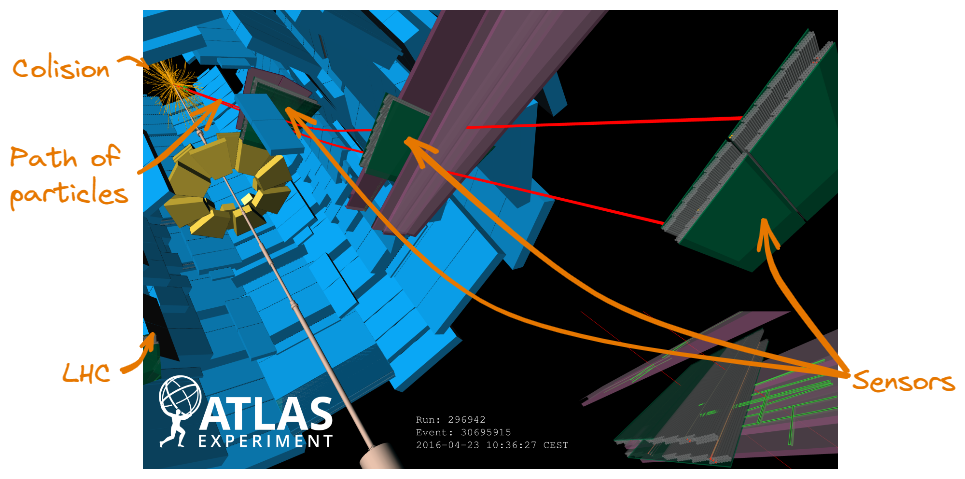
\includegraphics[width=0.85\textwidth]{05-resources/img/spec/experiment-atlas.excalidraw.png}
    \caption{ATLAS experiment at CERN~\cite{atlas-experiment}}
    \label{fig:introduction:particles:tracking}
\end{figure}

\section{Lawrence Berkeley National Laboratory}
\label{ch:introduction:lbl}

The \acrfull{lbl} is a national laboratory in Berkeley, California.
It is managed and operated by the University of California for the \acrfull{doe}.
The lab is situated in the hills of Berkeley and it is composed of many buildings
and has a beautiful view of the San Francisco Bay (see Fig.\ref{fig:introduction:lbl:view}).
This laboratory is mentioned in the recently released movie by Christopher Nolan,
"Oppenheimer".

\begin{figure}[ht]
    \centering
    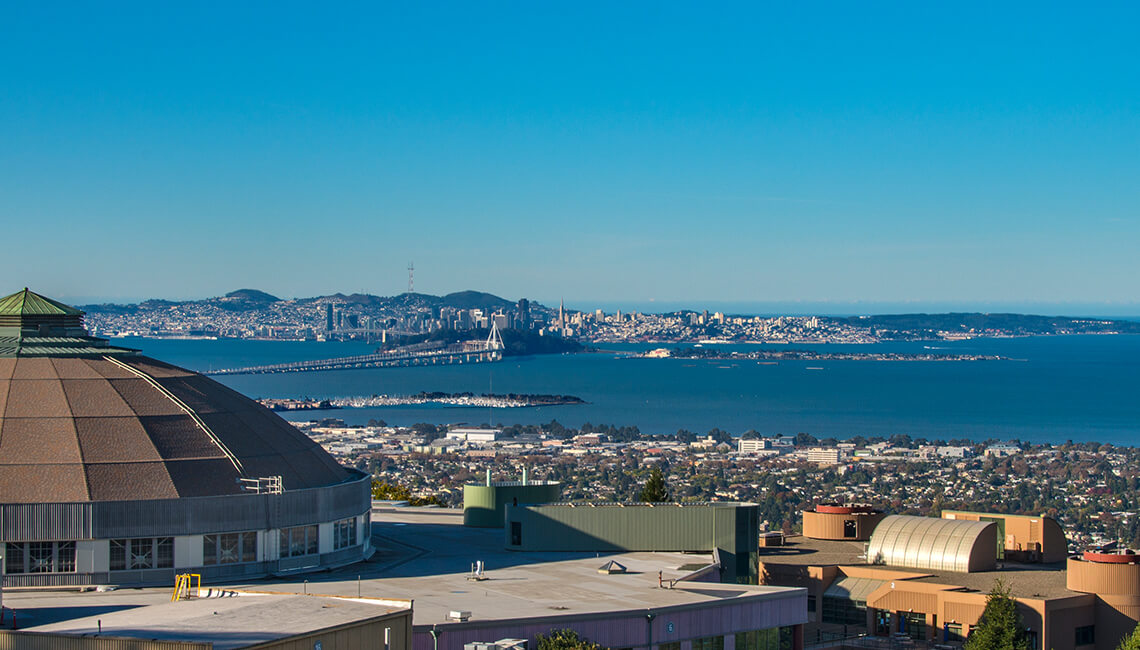
\includegraphics[width=0.8\textwidth]{05-resources/img/spec/lab-view.jpg}
    \caption{Lawrence Berkeley National Laboratory}
    \label{fig:introduction:lbl:view}
\end{figure}


\section{The objectives}
\label{ch:introduction:objectives}

Celeritas is already accelerated by \acrshort{gpu}s, however, the team wants to
improve the performance.
In the current version of the code, each particle track is processed in parallel
by one GPU thread, with no collaboration between threads.
GPU profiling of the code shows that execution time is dominated by two kernels.
The first one is handled by the interaction with the detector geometry to know
where, in 3D space, the particle is situated and during the profiling, the
library used is vecGeom~\cite{VecGeom}.
The second kernel, which will be the focus of this Bachelor thesis project, is
the computation of a differential equation using Dormand-Prince~\cite{princeDormand}.

However, the thesis can be a success even if the project doesn't meet the improvement.
This is because we don't yet know whether thread synchronization will be more
time-consuming than the original version.
In addition, the kernel launch in Celeritas have to be changed, and this
could take up a considerable amount of optimization time.
For the Bachelor thesis, it is sufficient to have a proof of concept that
demonstrates if the enhancement is effective and deserves to be integrated.
To measure the changes done during the internship, the profiler must be run
before and after each step of the project.
The mandatory requirements are described in the following section.

\subsection{Learn GPU programming}
\label{ch:introduction:objectives:learn-gpu-programming}

Before starting to work on the project, some things need to be learned and the goal here is to learn a new way of programming.
To conclude this goal, no code will be produced except for exercises, but the important notions of \acrshort{gpu} programming with CUDA will be synthesized using cheat sheets.
To take advantage of the delay between the beginning of the Bachelor thesis and the beginning of the \acrshort{lbl} internship, this step will be done during this time.


\subsection{Understand the project}
\label{ch:introduction:objectives:understand-the-project}

To be able to improve the performance of the code, the first step is to understand the project and it's always better to understand the background: why it is needed, who will use it and which paradigm and tools are used.

To measure the performance gained, it is necessary to know where the project is at each step.
To take a snapshot of the performance, a profiler can be run and this includes that we can compile and launch the project.
This step will be done at the beginning of the project on-site.


\subsection{Improve the performance}
\label{ch:introduction:objectives:improve-the-performance}

The main goal of the project is to improve the performance of the implementation of Dormand-Prince method~\cite{princeDormand}.
This last mandatory requirement is the core of the thesis and the most important part of the project and it will require the knowledge gained in the first two steps to improve the performance.

To conclude this step, the code must compile, pass the unit test, and a profiler must be run to show the difference between the new and the legacy implementation of the DormandPrince method.
To achieve this goal, the profiles must show an improvement, but this could meet some difficulties to be realized and integrated into the project.
In all cases, the failure of this goal doesn't mean the failure of the thesis if the documentation is correctly done and explains the results obtained and how is it possible or not to continue to this path.
This step will be done after the first two steps and it will take the whole time left.

\section{Optional requirements}
\label{ch:introduction:optional-requirements}

These optional goals are good additions to the project but they are not
require to have a concrete result.

The first one is to have a portable performance.
The purpose of Celeritas is to be run on all kinds of \acrshort{gpu} and even on machines with just a \acrshort{cpu}.
During the optimization, the improvement will be checked on the Perlmutter~\cite{Perlmutter} which uses Nvidia A100 with the architecture Ampere~\cite{ampere} and some improvement can be only effective to this kind of \acrshort{gpu}.
This goal is here to check if the improvement has a positive effect on other architectures and if it is not, to find a way to do that.
To begin this step, the main goal needs to be finished.

The second optional objective is to do another performance improvement.
If the performance of the Runge-Kutta method~\cite{Runge-Kutta-methods} is improved, another optimization can be done.
This part goal will be discussed further in the project with the supervisors and the customers and it will be managed like the last mandatory goal.
This step can be done multiple times if there is enough time.

\chapter{Analyze}
\label{ch:analyze}

During this chapter, the project is analyzed to understand the context, the
goals and challenges.
This project is focused on the optimization of the particle's tracking using
\acrshort{gpu}s.
The \acrshort{gpu}'s programming is something totally new for a bachelor's
student at the \acrshort{heia}.
Celeritas is a project that is actively developed and it requires time to
understand the code and the architecture.


\section{GPU}
\label{ch:analyze:gpu}

The \acrfull{gpu} is a processor that is specialized in parallel computing.
It is known by the gamer community because it is used to render the graphics of
the games and a good graphic card increases the frame per second displayed.
However, in the professional world, the \acrshort{gpu} are becoming more and
more popular because they are more efficient than the \acrshort{cpu} for
parallel computing and managing a large amount of data.


\subsection{Use cases}
\label{ch:analyze:gpu:use-cases}

In most of the case, \acrshort{cpu}s are more efficient than \acrshort{gpu}s
that is why they are a mandatory component of a computer.
\acrshort{cpu}s have a high frequency and they are optimized to execute one
task at a time with a high efficiency.
In the other hand, \acrshort{gpu}s have a lower frequency and they are optimized
to execute multiple tasks at the same time.

To understand, imagine John wants to eat dinner with his 5 kids and they have to
cook something and dress the table.
Cooking is a task that must be done sequentially and require some skills and
efficiency to be done quickly.
Dressing the table is a task where the skills don't affect the time but the
number of hands does.
This task can be done by the kids when everyone is putting something on the table.
In our case, John is the \acrshort{cpu} and the kids are the \acrshort{gpu}s.

The \acrshort{gpu}s are used when the number of workers is more important than
the efficiency of the worker like computing the pixels of an image or the
particles of a simulation.




\subsection{Architecture}
\label{ch:analyze:gpu:architecture}

The table \ref{tab:analyze:gpu:architecture:instruction-data} shows the
different types of processors.
The capabilities to work with one or multiple data and instructions are defined
by the architecture of the processor.

\begin{table}[ht]
    \centering
    \begin{tabular}{l|l|l|}
                          & Single data & Multiple data \\ \hline
    Single instruction    & SISD        & \textbf{SIMD}  \\ \hline
    Multiple instructions & MISD        & MIMD           \\ \hline
    \end{tabular}
    \caption{Different types of processors working with one or multiple data and instructions}
    \label{tab:analyze:gpu:architecture:instruction-data}
\end{table}

The \acrshort{gpu} is a \acrshort{simd} processor and the \acrshort{cpu} is a
\acrshort{sisd} processor.
The table \ref{tab:analyze:gpu:architecture:instruction-data} does not show the
frequency of the processor that is an important factor for the performance.
This explains why the \acrshort{cpu} is more efficient than the \acrshort{gpu}
for most of the cases.

To deal with the \acrshort{simd} architecture, the \acrshort{gpu} executed
physically the same instruction on multiple data using multiple threads as shown
on the figure \ref{fig:analyze:gpu:architecture:smid}.

\image{0.35}{05-resources/img/analyze/simd.png}
{SIMD physically executed}
{fig:analyze:gpu:architecture:smid}

The \acrshort{gpu} is composed of multiple \acrfull{sm} that are composed of
multiple \acrfull{cuda} cores.
The \acrshort{cuda} cores are the processors that execute the instructions.
The \acrshort{sm} is the unit that manages the threads and the memory.
\ref{fig:analyze:gpu:architecture:sm} shows the architecture of a \acrshort{sm}.

\image{0.65}{05-resources/img/analyze/sm.png}
{\acrshort{sm} architecture~\cite{nvidia-a100-architecture}}
{fig:analyze:gpu:architecture:sm}

The figure \ref{fig:analyze:gpu:architecture:sm} introduces the warp that is a
group of 32 threads that are executed in parallel.
The threads of a warp are linked together and they have to wait for the others
to finish their instructions.


\section{CUDA}
\label{ch:analyze:cuda}

\acrfull{cuda} is a parallel computing platform and programming model developed
by Nvidia.
It allows developers to use the \acrshort{gpu} to execute code written in C++, C, Fortran
and Python.
The \acrshort{cuda} platform is come with a \acrshort{sdk} that provides
libraries, debugging and profiling tools.

To develop with \acrshort{cuda}, the \acrshort{sdk} must be installed and all
the examples in this report are with C++ because it is the language used in the
project.

\subsection{Basis}
\label{ch:analyze:cuda:basis}

The code that runs on a \acrshort{gpu} is in a function called "kernel" and it
is executed by every thread.
Those kernels are defined with the keyword \texttt{\_\_global\_\_} and they are called
with the function \texttt{kernel\_name<<<number\_of\_blocks, number\_of\_threads>>>()}.
The code \ref{code:analyze:cuda:develop:basis:kernel} shows a basic kernel
launch with 2 blocks and 3 threads that say that the kernel code will be
executed 6 times.

\begin{code}
    \captionof{listing}{Basic kernel example}
    \label{code:analyze:cuda:basis:kernel}
    \begin{minted}{C++}
__global__ void kernel_name() {
    // Code executed on the device
}

int main() {
    // Code executed on the host
    kernel_name<<<2, 3>>>();
    return 0;
}
    \end{minted}
\end{code}

\subsection{Memory}
\label{ch:analyze:cuda:memory}

As the \acrshort{gpu} is a separate processor, it has its own memory system.
As a developer we have to manage three different spaces where data can be stored:
\begin{itemize}
    \item Host memory (RAM)
    \item Device memory (DRAM)
    \item Shared memory
\end{itemize}

Every space becomes with their properties and use the right one is important to
have a good performance.
The figure \ref{fig:analyze:cuda:memory:architecture} shows the physical
organization of the memory on a \acrshort{gpu}.

\image{1}{05-resources/img/analyze/gpu-memory.png}
{Physical memory organization on a \acrshort{gpu}~\cite{cuda-training}}
{fig:analyze:cuda:memory:architecture}


\subsubsection{Host memory}
\label{ch:analyze:cuda:memory:host}

Memory allocated on the host is the memory we use every day but it is not
accessible by the \acrshort{gpu}.
Even if a program is using the \acrshort{gpu}, it still needs to use the host
memory.

\subsubsection{Device memory}
\label{ch:analyze:cuda:memory:device}

The device memory is the memory that is used by the \acrshort{gpu} to execute
the kernel and it is comparable to a heap memory.
This place contains the local variables of a thread, the global variables and
the constant memory.
This memory is accessible by all the threads and the data could be loaded and saved
from the host.

The arguments passed to a kernel can only be 64 bytes long so the object must be
passed by reference and the value must be copied in the device memory.
To get the result, the data must be copied back to the host memory.
The code \ref{code:analyze:cuda:memory:device:copy-read} to launch a kernel
with objects and integers as arguments.
As the kernel isn't executed on the host, the return keyword can't be used to
get the result of the kernel so the result must be copied back to the host
using the same mechanism as the arguments.

\begin{code}
    \captionof{listing}{Load ang read data from the device memory}
    \label{code:analyze:cuda:memory:device:copy-read}
    \begin{minted}{C++}
__global__ void kernel_name(ObjectType1 *input1,
                            int input2,
                            ObjectType2 *output) {
    ObjectType3 local_variable;
    output[threadIdx.x] = ObjectType2(input1[threadIdx.x] + input2);
}

int main() {
    // Instantiate the variables
    ObjectType1 *h_input1, *d_input1;
    ObjectType2 *h_output, *d_output;

    // Setting the values
    h_input1 = new ObjectType1[100];
    for (int i = 0; i < 100; i++) {
        h_input1[i] = ObjectType1(i);
    }
    h_output = new ObjectType2[100];
    int input2 = 5;

    // Allocate the memory on the device
    cudaMalloc(&d_input1, 100 * sizeof(ObjectType1));
    cudaMalloc(&d_output, 100 * sizeof(ObjectType2));

    // Copy the data from the host to the device
    cudaMemcpy(d_input1,
               h_input1,
               100 * sizeof(ObjectType1),
               cudaMemcpyHostToDevice);

    // Launch the kernel
    kernel_name<<<1, 100>>>(d_input1, input2, d_output);

    // Copy the data from the device to the host
    cudaMemcpy(h_output,
               d_output,
               100 * sizeof(ObjectType2),
               cudaMemcpyDeviceToHost);

    // Free the memory
    cudaFree(d_input1);
    cudaFree(d_output);

    // Do something with the output
    print(h_output);

    return 0;
}
    \end{minted}
\end{code}

Constant expressions and method can be stored in the device memory using the
keyword \texttt{\_\_device\_\_}.
To keep a copy on the device, the double keyword
\texttt{\_\_host\_\_ \_\_device\_\_} could be used.


\subsubsection{Shared memory}
\label{ch:analyze:cuda:memory:shared}

The shared memory is a memory that is shared between the threads of a block.
It is quicker than the device memory but it is limited to 48~KB per block.
The shared memory is used to share data between the threads of a block and to
cache data from the global memory or exchange data between the threads.

The shared memory is allocated with the keyword \texttt{\_\_shared\_\_} and it
can be done statically~\ref{code:analyze:cuda:memory:shared:static} or
dynamically~\ref{code:analyze:cuda:memory:shared:dynamic}.
As the examples are very close of the code \ref{code:analyze:cuda:memory:device:copy-read},
the details to copy the data from the host to the device and from the device to
the host are not shown.

\begin{code}
    \captionof{listing}{Static shared memory allocation}
    \label{code:analyze:cuda:memory:shared:static}
    \begin{minted}{C++}
__global__ void kernel_name(ObjectType1 *input,
                            int input2,
                            ObjectType2 *output) {
    __shared__ ObjectType3 shared_variable[100];
    shared_variable[threadIdx.x] = ObjectType3(input[threadIdx.x] + input2);
    int index_next_thread = (threadIdx.x + 1) % 100;
    __syncthreads();
    output[threadIdx.x] = ObjectType2(shared_variable[index_next_thread]);
}

int main() {
    // Instantiate the variables
    // Setting the values
    // Allocate the memory on the device
    // Copy the data from the host to the device
    // Launch the kernel
    kernel_name<<<1, 100>>>(d_input1, input2, d_output);

    // Copy the data from the device to the host
    // Free the memory
    // Do something with the output
    return 0;
}
    \end{minted}
\end{code}

\begin{code}
    \captionof{listing}{Dynamic shared memory allocation}
    \label{code:analyze:cuda:memory:shared:dynamic}
    \begin{minted}{C++}
__global__ void kernel_name(ObjectType1 *input,
                            int input2,
                            ObjectType2 *output) {
    extern __shared__ ObjectType3 shared_variable[];
    shared_variable[threadIdx.x] = ObjectType3(input[threadIdx.x] + input2);
    int index_next_thread = (threadIdx.x + 1) % 100;
    __syncthreads();
    output[threadIdx.x] = ObjectType2(shared_variable[index_next_thread]);
}

int main() {
    // Instantiate the variables
    // Setting the values
    // Allocate the memory on the device
    // Copy the data from the host to the device
    // Compute the size of the shared memory
    int size_shared_memory = 100 * sizeof(ObjectType3);

    // Launch the kernel
    kernel_name<<<1, 100, size_shared_memory>>>(d_input1, input2, d_output);

    // Copy the data from the device to the host
    // Free the memory
    // Do something with the output
    return 0;
}
    \end{minted}
\end{code}


\subsection{Synchronization}
\label{ch:analyze:cuda:synchronization}

The easiest way to use \acrshort{gpu} is to have a set of data and using one
thread to update one data, for example there is the vector addition.
After, there are multiple dimension problems with matrix or bloc addition.
The most difficult type of problem is the reduction where the threads must
communicate between them to get the result. For example, the sum of all the
elements of a vector illustrated on the figure \ref{fig:analyze:cuda:synchronization:reduction}.

\image{0.5}{05-resources/img/analyze/reduction-problem.png}
{Reduction problem~\cite{cuda-training}}
{fig:analyze:cuda:synchronization:reduction}

\acrshort{cuda} provides some low-level function to synchronize, preserve the
integrity or exchanging the data.

\subsubsection{Atomic operations}
\label{ch:analyze:cuda:synchronization:atomic}

Atomic operations are used to preserve the integrity of the data when multiple
threads are trying to access the same data.
For example, if two threads are trying to increment a shared integer, the
result will be wrong because the two threads will read the same value and write
the same value so the result will be incremented only once.

Every atomic operation requires a pointer to the data that could eventually be
modified and a value.
The value could have different roles but the instruction is returning the old
value of the pointer.
The different atomic operations are listed on the table \ref{tab:analyze:cuda:synchronization:atomic}.

\begin{table}[ht]
    \centering
    \begin{tabular}{|m{0.5\textwidth}|m{0.4\textwidth}|}
        \hline
        \textbf{Operation} & \textbf{Description} \\
        \hline
        \texttt{atomicAdd/Sub(addr, val)} & Add a value to an integer \\
        \hline
        \texttt{atomicMin/Max(addr, val)} & Set the minimum/maximum value \\
        \hline
        \texttt{atomicInc/Dec(addr, val)} & Increment/Decrement an integer if the new value will be from 0 to val\\
        \hline
        \texttt{atomicCAS(addr, compare, val)} & Swap value to addr if old is equal to compare\\
        \hline
        \texttt{atomicExch(addr, val)} & Swap value to addr \\
        \hline
        \texttt{atomicAnd/Or/Xor(addr, val)} & Bitwise And/Or/Xor \\
        \hline
    \end{tabular}
    \captionof{table}{CUDA atomic operations}
    \label{tab:analyze:cuda:synchronization:atomic}
\end{table}

\subsubsection{Warp shuffle}
\label{ch:analyze:cuda:synchronization:warp-shuffle}

The warp shuffle is a function that allows developers to exchange data between the threads
of a warp.
This function is limiting the time waste to exchange data using shared memory
but it is only working for 4 or 8 bytes.

Those warp instructions are listed on the table \ref{tab:analyze:cuda:synchronization:warp-shuffle}.
They return the value of the variable specified from the thread lane specified.
The mask is a 32 unsigned bit that represents the lane-id in one-enabled bit.
Only the threads specified by this mask will be waited for the synchronization.
Var is the name of the variable that will be pulled from the thread lane.

\begin{table}[ht]
    \centering
    \begin{tabular}{|m{0.5\textwidth}|m{0.4\textwidth}|}
        \hline
        \textbf{Operation} & \textbf{Description} \\
        \hline
        \texttt{\_\_shfl\_sync(mask, var, lane)} & Get the value from the thread lane\\
        \hline
        \texttt{\_\_shfl\_up/down\_sync(mask, var, delta)} & Get the value from the thread lane $\pm$ delta\\
        \hline
        \texttt{\_\_shfl\_xor\_sync(mask, var, laneMask)} & Get the value from the thread lane \^{} laneMask\\
        \hline
    \end{tabular}
    \captionof{table}{CUDA warp shuffle operations}
    \label{tab:analyze:cuda:synchronization:warp-shuffle}
\end{table}


\subsubsection{Sync}
\label{ch:analyze:cuda:synchronization:sync}

Warp shuffle offer a synchronization method but \acrshort{cuda} provides
functions to synchronize the threads.
This could be useful if the threads have to exchange data between them using
the shared memory.

The table \ref{tab:analyze:cuda:synchronization:sync} shows the different
synchronization functions.

\begin{table}[ht]
    \centering
    \begin{tabular}{|m{0.5\textwidth}|m{0.4\textwidth}|}
        \hline
        \textbf{Operation} & \textbf{Description} \\
        \hline
        \texttt{\_\_syncthreads()} & Synchronize all the threads of a block\\
        \hline
        \texttt{\_\_threadfence()} & Synchronize all memory access of a block\\
        \hline
        \texttt{\_\_synchwarp(mask)} & Synchronize the threads of a warp that match the mask (default: all)\\
        \hline
    \end{tabular}
    \captionof{table}{CUDA synchronization functions}
    \label{tab:analyze:cuda:synchronization:sync}
\end{table}


\subsection{Create a project with CUDA}
\label{ch:analyze:cuda:create_project}

\acrshort{cuda} programming can be easily integrated in any C++ project.
The most constraint is to have a \acrshort{gpu} to execute the code and it is
easy to build on them to be sure that version is the same.
If the working station doesn't have a \acrshort{gpu}, it is possible to use a
SSH connection to a server with a \acrshort{gpu}.

To do that with CLion, the first step is to have a project and then in the
settings, add a toolchain with the \acrshort{cuda} compiler~\ref{fig:analyze:cuda:toolchain}.
Then in the CMake profile set the toolchain set before~\ref{fig:analyze:cuda:profile}.

Usually, the kernels are defined in a \texttt{.cu} file and the host code is in
a \texttt{.cc} file but everything can be in the same file.
To run the code, the most convenient way is to use CMake to compile the code
and then run the executable.
The code \ref{code:analyze:cuda:create_project} shows a basic CMake file to
compile a project with \acrshort{cuda}.

\begin{code}
    \captionof{listing}{Basic CMake file to compile a project with CUDA}
    \label{code:analyze:cuda:create_project}
    \begin{minted}{CMake}
cmake_minimum_required(VERSION 3.16)
project(project_name LANGUAGES CXX CUDA)

set(CMAKE_CXX_STANDARD 14)

# add CUDA
find_package(CUDA REQUIRED)

# add executable
add_executable(executable_name executable_file.cu)
    \end{minted}
\end{code}

\image{0.8}{05-resources/img/analyze/clion-toolchain.png}
{Add CUDA toolchain}
{fig:analyze:cuda:toolchain}

\image{0.8}{05-resources/img/analyze/cmake-profile.png}
{Set profile to toolchain}
{fig:analyze:cuda:profile}



\section{Celeritas}
\label{ch:analyze:atlas}

Celeritas is a \acrfull{hep} detector simulation on \acrshort{gpu}s started
early 2020.
This project is to respond to the large amount of data produced by the
\acrfull{lhc} that is not possible to be processed by traditional
\acrshort{cpu}s.
The project is actively developed by five laboratories that are: \acrfull{lbl},
\acrfull{ornl}, \acrfull{anl}, \acrfull{fnal} and \acrfull{bnl}.
The code leader is Seth Johnson from \acrshort{ornl} and Julien Esseiva is the only
participant from the \acrshort{lbl}.

\image{0.75}{05-resources/img/analyze/celeritas-organization.png}
{Celeritas actors and roles~\cite{celeritas-presentation-johnson}}
{fig:analyze:atlas:organization}

The goal is to simulate electromagnetic physics for the \acrshort{lhc} detectors
with the same precision.
The application could act as a plugin for Geant4, or a standalone application.


\subsection{Geant4}
\label{ch:analyze:atlas:geant4}

Celeritas has an end-to-end solution that can be launched standalone.
This version allows the developer to have a full control on the simulation
workflow and choose the geometry motors and physics models.
However, the standalone version needs a lot of development to be as complete as
Geant4.

\image{1}{05-resources/img/analyze/celeritas-end2end-integration.png}
{Integration diagram of the standalone application~\cite{celeritas-overview-tognini}}
{fig:analyze:atlas:geant4:end2end}


Celeritas has a version called "Acceleritas" that have the same code base as the
standalone version but it is used as a Geant4 plugin.
This version provides less improvement but all the Geant4's features are available.

\image{1}{05-resources/img/analyze/celeritas-acceleritas-integration.png}
    {Integration diagram for overloading of Geant4~\cite{celeritas-overview-tognini}}
    {fig:analyze:atlas:geant4:plugin}

Geant4~\cite{geant4} is a toolkit for the simulate the path of particles through
matter.
It is used in a multiple of fields, including the experiments made in the
accelerator physics.
This tool is developed by the \acrfull{cern} and is currently used by the
\acrfull{atlas} and \acrfull{cms} experiments.


\subsection{Runge Kutta Dormand Prince}
\label{ch:analyze:atlas:rkdp}

The \acrfull{rkdp} is a numerical method to solve ordinary differential equations.
It uses the coefficients from the Butcher tableau which is a low triangular
matrix.
The method is used to simulate the path of a particle through matter and
magnetic fields to a boundary of a sensor.

This is the Butcher tableau~\ref{tab:analyze:atlas:rkdp:butcher} for the \acrshort{rkdp} used in Celeritas.

\begin{table}[ht]
    \resizebox{\textwidth}{!}{
        \begin{tabular}{c|ccccccc}
            0    &            &             &            &          &               &          &      \\
            1/5  & 1/5        &             &            &          &               &          &      \\
            3/10 & 3/40       & 9/40        &            &          &               &          &      \\
            4/5  & 44/45      & -56/15      & 32/9       &          &               &          &      \\
            8/9  & 19372/6561 & -25360/2187 & 64448/6561 & -212/729 &               &          &      \\
            1    & 9017/3168  & -355/33     & 46732/5247 & 49/176   & -5103/18656   &          &      \\
            1    & 35/384     & 0           & 500/1113   & 125/192  & -2187/6784    & 11/84    &      \\
            \hline
                 & 35/384     & 0           & 500/1113   & 125/192  & -2187/6784    & 11/84    & 0    \\
                 & 5179/57600 & 0           & 7571/16695 & 393/640  & -92097/339200 & 187/2100 & 1/40 \\
        \end{tabular}
    }
    \captionof{table}{Butcher tableau for the \acrshort{rkdp}}
    \label{tab:analyze:atlas:rkdp:butcher}
\end{table}



\subsection{Particle's path}
\label{ch:analyze:atlas:path}

Celeritas simulates the path of a particle through matter and magnetic fields.
The path of a particle is calculated by the \acrshort{rkdp}~\ref{ch:analyze:atlas:rkdp} method.

\todo{add an image a particle's path}

As Celeritas is actively developed, not all the particles are now implemented.
The team focused on the High Luminance experiments and the particles that are
implemented are listed in the table \ref{tab:analyze:atlas:particles:implemented}.

\begin{table}[ht]
    \centering
    \begin{tabular}{lll}
        \hline
        \textbf{Particle}         & \textbf{Process}     & \textbf{Model(s)}            \\
        \hline
        \multirow{4}{*}{$\gamma$} & photon conversion    & Bethe—Heitler                \\
                                  & Compton scattering   & Klein—Nishina                \\
                                  & photoelectric effect & Livermore                    \\
                                  & Rayleigh scattering  & Livermore                    \\
        \hline
        \multirow{4}{*}{$e^\pm$}  & ionization           & Mø11er-Bhabha                \\
                                  & bremsstrahlung       & Seltzer—Berger, relativistic \\
                                  & pair annihilation    & EPlusGG                      \\
                                  & multiple scattering  & Urban, WentzelV1             \\
        \hline
        $\mu^\pm$                 & muon                 & Muon Bremsstrahlung          \\
        \hline
    \end{tabular}
    \captionof{table}{Particles now implemented in Celeritas~\cite{exasclae-computing-ornl-evans}}
    \label{tab:analyze:atlas:particles:implemented}
\end{table}

The team is working on expand the project to other experiments and have planned
to add the following particles~\ref{tab:analyze:atlas:particles:planned}.

\begin{table}[ht]
    \centering
    \begin{tabular}{lll}
        \hline
        \textbf{Physics}          & \textbf{Process}       & \textbf{Particle(s)}              \\
        \hline
        \multirow{10}{*}{EM}      & Photon conversion      & $\gamma$                          \\
                                & pair annihilation      & $e^\pm$                           \\
                                & photoelectric effect   & $\gamma$                          \\
                                & ionization             & charged leptons, hadrons and ions \\
                                & bremsstrahlung         & charged leptons and hadrons       \\
                                & Rayleigh scattering    & $\gamma$                          \\
                                & Compton scattering     & $\gamma$                          \\
                                & Coulomb scattering     & charged leptons and hadrons       \\
                                & multiple scattering    & charged leptons and hadrons       \\
                                & continuous energy loss & charged leptons, hadrons and ions \\
        \hline
        \multirow{3}{*}{Decay}    & two body decay         & $\mu^\pm$, $\tau^\pm$, hadrons    \\
                                & three body decay       & $\mu^\pm$, $\tau^\pm$, hadrons    \\
                                & n-body decay           & $\mu^\pm$, $\tau^\pm$, hadrons    \\
        \hline
        \multirow{6}{*}{Hadronic} & photon-nucleus         & $\gamma$                          \\
                                & lepto-nucleus          & leptons                           \\
                                & nucleon-nucleon        & $p$, $n$                          \\
                                & hadron-nucleon         & hadrons                           \\
                                & hadron-nucleus         & hadrons                           \\
                                & nucleus-nucleus        & hadrons                           \\
        \hline
    \end{tabular}
    \caption{Particles planned in the future version of Celeritas~\cite{exasclae-computing-ornl-evans}}
    \label{tab:analyze:atlas:particles:planned}
\end{table}


\subsection{Implementation}
\label{ch:analyze:atlas:implementation}

Celeritas is realized in C++ and uses CUDA, HIP or OpenMP to accelerate the
simulation.
The code is data-oriented and is using composition instead of inheritance, and
to optimize the kernel launching on the \acrshort{gpu}, all the data are loaded
one time at the beginning of the simulation.

Celeritas is using a flow of action to process the data given, compute the
tracks, simulate the collisions and finally return the results as shown in the
figure \ref{fig:analyze:atlas:implementation:activity-diagram-gpu-topological}.

\image{0.75}{05-resources/img/analyze/celeritas-GPU-loop-topological.png}
{Celeritas's actions activity diagram~\cite{chep2023-presentation-johnson}}
{fig:analyze:atlas:implementation:activity-diagram-gpu-topological}

The project is focusing on optimizing a part of the particles' tracking which is
made in the action called "Along Step".
This action is executed for each particle by one dedicated \acrshort{gpu}'s
thread.
The figure \ref{fig:analyze:atlas:implementation:activity-diagram-track} shows
the activity diagram of the particle's track.

\image{0.5}{05-resources/img/analyze/activity-diagram-track.png}
{Activity diagram of a particle's track~\cite{atlas-week-esseiva}}
{fig:analyze:atlas:implementation:activity-diagram-track}

The method \acrshort{rkdp}~\ref{ch:analyze:atlas:rkdp} is used to calculate the
chord of the path during the action "Calculate substep from remaining distance"
in the figure \ref{fig:analyze:atlas:implementation:activity-diagram-track}.
The chord, with a different step's size, is computed until the error meets the tolerance or the number of try
is reached.
If the tolerance is not met, an ultimate iteration will be made and the error
is provided.

According to the result of an experiment made by the \acrfull{cms} and the
graphics \ref{fig:analyze:atlas:implementation:iteration-hit} show that in more than 80\% of the cases, the tolerance is
met at the first iteration.

\image{1}{05-resources/img/analyze/celeritas-iteration-hit.png}
{Number of iterations needed to meet the tolerance for each computed chord}
{fig:analyze:atlas:implementation:iteration-hit}

\subsection{Optimization}
\label{ch:analyze:atlas:optimization}

Celeritas is already accelerated by \acrshort{gpu}s, but the performance could
be improved.

To simulate the particles, Celeritas uses one thread to track one particle.
The team wants to improve the performances by using more than one thread per
track.
During the simulation, the \acrfull{rkdp} is used multiple times to calculate
the position of the particle.

\image{0.5}{05-resources/img/analyze/celeritas-optimization.png}
{Celeritas runtime per action~\cite{chep2023-presentation-johnson}}
{fig:analyze:atlas:optimization:celeritas-optimization}





\section{Images Backup}
\label{ch:analyze:images}

\image{0.5}{05-resources/img/analyze/celeritas-GPU-loop-branch.png}
{Celeritas activity diagram for the GPU loop (Source: Seth Johnson https://github.com/celeritas-project/celeritas-docs/blob/main/presentations/chep-2023/srj-chep.pdf)}
{fig:analyze:atlas:implementation:activity-diagram-gpu}

\image{0.5}{05-resources/img/analyze/field-propagator-near-miss.png}
{Path simulation with chord (Source: Set Johnson https://github.com/celeritas-project/celeritas-docs/blob/main/presentations/doe-briefing-20201019/pres.pdf)}
{fig:analyze:atlas:implementation:field-propagator-near-miss}

\image{0.5}{05-resources/img/analyze/celeritas-kernel.png}
{Detail of the kernels (Source Seth Johnson https://github.com/celeritas-project/celeritas-docs/blob/main/presentations/geant4-collab-202209/Celeritas.pdf)}
{fig:analyze:atlas:implementation:kernel}

\image{0.5}{05-resources/img/analyze/celeritas-gpu-algorithm.png}
{GPU algorithm (Source: Seth Johnson https://github.com/celeritas-project/celeritas-docs/blob/main/presentations/lbnl-202302/srj-lbnl-2023.pdf)}
{fig:analyze:atlas:implementation:gpu-algorithm}

\chapter{Design}
\label{ch:design}

This bachelor thesis is focusing on optimizing the \acrlong{rkdp} algorithm
in a context of \acrshort{gpu} computing.
The design of the project amounts to find possible adaptations that could
decrease the execution time of the algorithm.

\section{Simulation}
\label{ch:design:simulation}

\acrshort{rkdp} is a sequential function and as it is described in Chapter~\ref{ch:analyze:gpu:use-cases},
\acrshort{gpu}s or parallelization is not so useful in this case.
This simulation aims at estimating to what extent using multithreading could
potentially improve the running time.

\subsection{RKDP algorithm}
\label{ch:design:simulation:rkdp}

This method has nine stages and is a fifth-order accurate Runge Kutta method.
The first six stages are used to compute the end state, the seventh stage is used
in the seventh state and the last two stages are used to compute the error and the
middle state.

\subsection{Principle}
\label{ch:design:simulation:principle}

In the implementation of the \acrshort{rkdp}, we can identify different types of
code.
The first category must is the code that must be executed sequentially and has no option
to be distributed on multiple threads.
The second group of concern is the code that concerns the computation of several
expressions that must be assigned before the first reference to the
corresponding variables.
The last one is a vector multiplication that has a specified place in the code
but could be split into parallel substeps.

Figure \ref{fig:design:simulation:principle:code-type} shows how the
fourth step is computed and which part of the code is from which type.
The red part is the dependent code, that has to be executed sequentially.
It is the computation of the intermediate state kx using the equation.
The blue part is the independent code that just has to be executed before its
first use. This is the computation of the coefficients with the step's size.
The green part is the vector multiplication that can be executed in parallel.
Each line has to be computed sequentially but each involves a vector
multiplication which could be multithreaded.
Code~\ref{code:design:simulation:principle:axpy} shows the implementation of the
method

\image{0.5}{05-resources/img/design/simulation-principle.excalidraw.png}
        {Example illustrating which part of the code is from which type}
        {fig:design:simulation:principle:code-type}

\begin{code}
    \captionof{listing}{Implementation of axpy}
    \label{code:design:simulation:principle:axpy}
    \begin{minted}{c++}
//! \file celeritas/field/Types.hh
/*!
* Perform y <- ax + y for OdeState.
*/
inline CELER_FUNCTION void axpy(real_type a, OdeState const& x, OdeState* y)
{
    axpy(a, x.pos, &y->pos);
    axpy(a, x.mom, &y->mom);
}
//----------------------------------------------------------------------------//
//! \file celeritas/ext/Convert.geant.hh
/*!
 * Define y += a * x .
 */
inline void axpy(double a, G4ThreeVector const& x, G4ThreeVector* y)
{
    CELER_EXPECT(y);
    for (int i = 0; i < 3; ++i)
    {
        (*y)[i] = a * x[i] + (*y)[i];
    }
}
    \end{minted}
\end{code}

The principle is to record when what type of code is executed to have an idea of
the proportion of time spent on each type of code.
Code \ref{code:design:simulation:principle:code} shows the same step as
Figure \ref{fig:design:simulation:principle:code-type} but with the
logger to record the type of code, and written in Python.

\begin{code}
    \captionof{listing}{Fourth step in Python for the simulation}
    \label{code:design:simulation:principle:code}
    \begin{minted}{python}
# Fourth step
logger(4, TaskType.DEPENDENT)
k4 = equation(*state)
state = beg_state
logger(4, TaskType.INDEPENDENT)
coef_a41 = step * a41
coef_a42 = step * a42
coef_a43 = step * a43
coef_a44 = step * a44
logger(4, TaskType.VECTOR_MULT)
axpy(coef_a41, k1, state)
axpy(coef_a42, k2, state)
axpy(coef_a43, k3, state)
axpy(coef_a44, k4, state)
    \end{minted}
\end{code}

The logger is an object that creates an event with a type and a timestamp.
This object is used during the runtime but also after to display the results and
to compute the better thread workload using a \texttt{SchedulingTree} described
in the next section~\ref{ch:design:simulation:scheduling}.

\subsection{SchedulingTree}
\label{ch:design:simulation:scheduling}

The \texttt{SchedulingTree} has been developed to compute the ideal start time
for a given task with the best wanted time.

To choose which task will be executed on which thread, we ask every thread,
which are represented by a \texttt{SchedulingTree}, to know which thread could
start the thread with the best time.
When the best thread is found, the task is added to it.

The implementation is inspired by an interval tree.
The tasks are the leaf and every node has the same start as the left child and
the same end as the right child.
This allows the code to know if a task could potentially overlap an existing one.
To get the result, the leaves have to be read from the left to the right.
The tasks are only stocked in the leaves and the node is only used to know if a
new task could potentially overlap an existing one.
Figure~\ref{fig:design:simulation:scheduling:schema} shows an example of a
\texttt{SchedulingTree} with three tasks.
The node help to have a quick overview if a task could overlap and existing or
not.

\image{0.5}{05-resources/img/design/schedulingTree.excalidraw.png}
        {Example of a \texttt{SchedulingTree} with three tasks}
        {fig:design:simulation:scheduling:schema}

The \acrshort{api} of the \texttt{SchedulingTree} is shown in Table~\ref{tab:design:simulation:scheduling:api}.
The implementation is not user-bad-usage-proof because indicating an invalidate
start time in the method \texttt{add} will result in the overlapping of some
tasks.

\begin{table}[ht]
    \centering
    \begin{tabular}{|m{0.45\textwidth}|m{0.45\textwidth}|}
        \hline
        \textbf{Method} & \textbf{Description} \\
        \hline
        \texttt{schedule(int wanted\_start, Task task) -> int} & Return the earliest start possible after the wanted start given in the parameter \\
        \hline
        \texttt{add(int start, Task task) -> void} & Add a task at the time indicated in the parameter \\
        \hline
        \texttt{get\_schedule() -> Task[]} & Return the array of the tasks sorted by start time \\
        \hline
    \end{tabular}
    \captionof{table}{\acrshort{api} of the \texttt{SchedulingTree}}
    \label{tab:design:simulation:scheduling:api}
\end{table}

\subsection{Results}
\label{ch:design:simulation:results}

Those results are obtained by recording the data from a Python script running
the \acrshort{rkdp} with the chaotic Lorenz attractor equation.

The second graph of Figure \ref{fig:design:simulation:results} shows
how the time is spent in each step.
This version is without some dead time that appears when recording the events.
It is important to have this version because when we are simulating the
distribution on the threads, we are not taking into account the dead time.

The graphs three and four are showing what each thread is doing.
We can see that pre-computing the coefficients with the three threads when the
first one is computing the equation seems to be a good idea.
Also, distributing the vector multiplication could help a lot to decrease the
execution time.

The last graph is like the first two ones but with the new repartition of the
tasks.

To conclude, this simulation shows that we can expect an improvement in dividing
the time up by two.
However, this simulation is not taking the time due to the thread
synchronization and it is run in a different context than the real implementation.

To implement this solution, the workload has to be divided between the threads.
According to the result, the best workload would be something like Figure~\ref{fig:design:simulation:result:thread-workload}.
Where a controller is computing the intermediate state using the equation and the
other threads are computing the vector multiplication.
The role of the threads has been slightly adapted from graph number three and
four of Figure~\ref{fig:design:simulation:results}.

\image{0.5}{05-resources/img/design/thread-workload.excalidraw.png}
        {Best theoretical distribution of the workload between the threads}
        {fig:design:simulation:result:thread-workload}

\image{1}{05-resources/img/design/simulation-result.png}
        {Results of the simulation}
        {fig:design:simulation:results}


\section{Shared memory management}
\label{ch:design:shared}

The allocation of the shared memory is a part of some implementations of the
new \acrshort{rkdp}.
To use this memory, the developer must deal with constraints about the size and
the alignment of the data.

For each track, the shared must contain eight \texttt{OdeState} and one
\texttt{FieldStepperResult}. The \texttt{OdeState}s are the seven intermediate
states (kx) and the last one is the state that is updated during the
whole method (along\_state).
If the coefficients are pre-computed using multiple threads, they also have to be
stored in the shared memory.
Table~\ref{tab:design:shared-component} shows the size of each objects for a
track.

\begin{table}[ht]
    \centering
    \begin{tabular}{|l|l|l|}
        \hline
        \textbf{Variable} & \textbf{Type} & \textbf{Size (bytes)} \\
        \hline
        ks & OdeState[7] & 45 * 7 = 315 \\
        \hline
        along\_state & OdeState & 45 \\
        \hline
        result & FieldStepperResult & 144 \\
        \hline
        (coef) & double[32] & 8 * 32 = 256 \\
        \hline
        \multicolumn{2}{|l|}{Total} & 528 (784) \\
        \hline
    \end{tabular}
    \captionof{table}{Objects stored in the shared memory for each track}
    \label{tab:design:shared-component}
\end{table}

According to Table~\ref{tab:design:shared-component}, the block size
has a maximum dimension of 372 threads for the version without precomputed (Equation~\ref{eq:design:shared:dimension-without-coef})
and 248 threads for the version with precomputed coefficients (Equation~\ref{eq:design:shared:dimension-with-coef}).

\begin{equation}
    \frac{49152\frac{B}{Block} }{528 \frac{B}{Track} } * 4 \frac{Thread}{Track} = 93\frac{Track}{Block} * 4 \frac{Thread}{Track} = \textbf{372}\frac{Thread}{Block}
    \label{eq:design:shared:dimension-without-coef}
\end{equation}

\begin{equation}
    \frac{49152\frac{B}{Block} }{784 \frac{B}{Track} } * 4 \frac{Thread}{Track} = 62\frac{Track}{Block} * 4 \frac{Thread}{Track} = \textbf{248}\frac{Thread}{Block}
    \label{eq:design:shared:dimension-with-coef}
\end{equation}

However, the shared memory size is not the only constraint.
The shared memory can be allocated statically or dynamically.
In this project, the number of tracks is not known at compile time so it is
mandatory to use a dynamic allocation.
The easiest way to do this is to have an array of different types of objects and
use the thread id as an index to access the data as shown in Figure~\ref{fig:design:shared:memory-organization}.

\image{1}{05-resources/img/design/memory-management.excalidraw.png}
        {Shared memory management}
        {fig:design:shared:memory-organization}

Assuming that the shared memory is a big array of void pointers and knowing the
number of tracks of the block, it is possible to create aligned pointers to the
different objects.
The operator \texttt{[x]} on a pointer is returning the pointer to the address
\texttt{ptr + x * sizeof(type)}. So using \texttt{[n]} is giving the first
address of the next array.


\section{Number of iterations}
\label{ch:design:iterations}

As shown in the Chapter~\ref{ch:analyze:atlas:implementation} and Figure~\ref{fig:analyze:atlas:implementation:iteration-hit},
more than 80\% of the time concerns just one iteration.
However, this does not take into account the time spent to get these results.
For example, if a chord needs 100 iterations, it has taken 100 times more time
than a chord that needs only one iteration.
To have a better view of the effort that takes an iteration, the data have been
multiplied by the number of iterations.
The result is shown in Figure~\ref{fig:design:iterations:iteration-hit}.

\image{1}{05-resources/img/design/time-iteration-hit.png}
        {Time before an iteration is hit multiplied by the number of iterations to
        have an idea of the time spent in each iteration.}
        {fig:design:iterations:iteration-hit}

As we can see, the first iteration is still the most used.
However, there is a better distribution and we can't assume that doing only one
iteration during the test is representative of the real use of the algorithm.

Based on the heuristic rule of the 80/20, a good number of iterations
will be a number that represents 80\% of the time.
Figure~\ref{fig:design:iterations:cumulative-time} shows that this number
is 40 iterations.

\image{0.5}{05-resources/img/design/cumulative-time-iteration.png}
        {Cumulative percentage of the time spent in the iterations with a marker
        at 80\%.}
        {fig:design:iterations:cumulative-time}
\chapter{Implementation}
\label{ch:implementation}

The implementation of this Bachelor thesis is not done from scratch, it is the
improving the Celeritas project.
My contribution is detailed in a pull request available here~\cite{pull-request-barras}.


\section{Project initialization}
\label{ch:implementation:initialization}

Before actively developing the project, it is necessary to set up the
environment, compile the project and run it to ensure that everything is
working as expected.

\subsection{Set up the environment}
\label{ch:implementation:initialization:environment}

This project is designed to be run on \acrshort{hpc}.
This means that the tools are slightly different from a regular project.
Those systems are designed to be used by multiple users at the same time.
Therefore, they have to be adapted to any usage and provide the needed tools
or libraries that the users want.
To help the users, the system provides a module system or an advanced package
manager like \texttt{spack}~\cite{Spack}.


\subsubsection{Module system}
\label{ch:implementation:initialization:environment:module}

Module~\cite{Module} is a tool that allows the user to load or unload some tools
or libraries.
It is a simple way to manage the environment and it must be installed and
managed by the system administrator.

Table~\ref{tab:implementation:initialization:environment:module:commands} shows
some commands that can be used with the module system.
They are basic but they are sufficient in most cases.

\begin{table}[ht]
    \centering
    \begin{tabular}{|l|l|}
        \hline
        \textbf{Command} & \textbf{Description} \\
        \hline
        \texttt{module avail} & List all available module \\
        \hline
        \texttt{module list} & List all loaded module \\
        \hline
        \texttt{module load <module>} & Load a module \\
        \hline
        \texttt{module unload <module>} & Unload a module \\
        \hline
    \end{tabular}
    \caption{List of useful modules commands}
    \label{tab:implementation:initialization:environment:module:commands}
\end{table}

The command can be added to the profile to load a module when a session is open,
for example, \texttt{module load git}.


\subsubsection{Spack}
\label{ch:implementation:initialization:environment:spack}

Spack~\cite{Spack} is an advanced package manager designed for \acrshort{hpc} applications.
This tool can be installed by the user and it helps to install some projects like
Celeritas with their dependencies.
Like module, spack allows the user to work on many different projects with the
system of the environment.

Install this tool, it requires to clone the repository and source it.
As sourcing a script is shell session scoped, it is recommended to add it to the
profile.
Code~\ref{code:implementation:initialization:environment:spack:install} shows

\begin{code}
    \captionof{listing}{Download spack and source it}
    \label{code:implementation:initialization:environment:spack:install}
    \begin{minted}{bash}
git clone\
    --depth=100\
    --branch=releases/v0.20 https://github.com/spack/spack.git\
    ~/spack

echo ". ~/spack/share/spack/setup-env.sh" >> ~/.bashrc
    \end{minted}
\end{code}

To reload the profile, use the command \texttt{source ~/.bashrc}.

\begin{table}[ht]
    \centering
    \begin{tabular}{|m{0.45\textwidth}|m{0.45\textwidth}|}
        \hline
        \textbf{Command} & \textbf{Description} \\
        \hline
        \texttt{spack env create <name> <path>} & Create a new environment based
            on a YAML file that describes the environment \\
        \hline
        \texttt{spack env activate <name>} & Activate an environment \\
        \hline
        \texttt{spack env deactivate} & Deactivate the current environment \\
        \hline
        \texttt{spack env list} & List all environments \\
        \hline
        \texttt{spack env remove <name>} & Remove an environment \\
        \hline
        \texttt{spack concretize -f} & Show what will be installed with which option.
            This command is very useful to check that spack will install
            Celeritas with the \acrshort{gpu} acceleration \\
        \hline
        \texttt{spack install} & Install the environment \\
        \hline
        \texttt{spack find} & List all installed packages \\
        \hline
        \texttt{spack config add package:all:variants:"+/-option"} & Add a variant to all packages \\
        \hline
    \end{tabular}
    \caption{List of useful spack commands}
    \label{tab:implementation:initialization:environment:spack:commands}
\end{table}


\subsubsection{Celeritas environment}
\label{ch:implementation:initialization:environment:celeritas}

As shown in the previous sections, the environment is something important and
it needs a bit of a configuration to have the right one.
Code \ref{code:implementation:initialization:environment:celeritas:create} is
the profile used to develop the project on the host Zeus.
It assumes that the environment \texttt{celeritas} has already been created with spack.

\begin{code}
    \captionof{listing}{Profile to work with Celeritas}
    \label{code:implementation:initialization:environment:celeritas:create}
    \begin{minted}{bash}
# Load spack
. ~/spack/share/spack/setup-env.sh
# Load the right compiler (Zeus)
module unload gcc
source /cvmfs/sft.cern.ch/lcg/contrib/gcc/11.3.0/x86_64-centos7-gcc11-opt/setup.sh
# Activate the environment (Optional)
spack env activate celeritas
    \end{minted}
\end{code}


\subsection{Compile the project}
\label{ch:implementation:initialization:compile}

Celeritas is a complex project with multiple builds possible.
The easiest way to compile it is to use the script provided by the team here:
\texttt{./scripts/build.sh}.
This script will automatically read the host to load the right compiler, the
right modules and the right Cmake profile.
In the end, this script will build all the applications issued from this project
and run the tests.
This script is loading the Cmake preset and his name must be given as an
argument.
Code~\ref{code:implementation:initialization:compile:presets} lists all the
available presets.

\begin{code}
    \captionof{listing}{Cmake preset for Celeritas}
    \label{code:implementation:initialization:compile:presets}
    \begin{minted}{bash}
Sourcing environment script at scripts/env/zeus.sh
loading cuda/11.8.0
Usage: scripts/build.sh PRESET [config_args...]
Available configure preses:

    "base"        - Zeus default options (GCC, debug)
    "reldeb-novg" - Zeus release with debug symbols and Orange
    "reldeb"      - Zeus release with debug symbols
    "ndebug-novg" - Zeus release with Orange
    "ndebug"      - Zeus release
    "default"     - Automatic options (debug with tests)
    "full"        - Full
    "minimal"     - Minimal
    \end{minted}
\end{code}

If this is the first time the project is built, some pre-steps are required.
To start, the right compiler must be loaded.
Then, the spack environment must be created.
Code~\ref{code:implementation:initialization:compile:pre-steps} shows those two
parts.

\begin{code}
    \captionof{listing}{Pre-steps to compile Celeritas}
    \label{code:implementation:initialization:compile:pre-steps}
    \begin{minted}{bash}
## Load the right compiler (Zeus) ##
module load cmake
module unload gcc
source /cvmfs/sft.cern.ch/lcg/contrib/gcc/11.3.0/x86_64-centos7-gcc11-opt/setup.sh

## Create the environment ##
# Configure the project to be used with CUDA
spack config add packages:all:variants:"+cuda cuda_arch=80"
spack env create celeritas scripts/spack.yaml
spack activate celeritas
    \end{minted}
\end{code}

After this step, it just needs to install the environment using
\texttt{spack install} (can be parallelized with \texttt{spack install \& spack install \& ...})
but this step takes a couple of hours.
To avoid doing that multiple times, it is recommended to use the command
\texttt{spack concretize -f} to check what environment will be installed.
The important thing is to have \texttt{vecgeom} compiled with \texttt{gcc 11.3}
and have the variant \texttt{cuda} enabled with the architecture \texttt{80} for
Zeus and \texttt{70} for Perlmutter.
During this Bachelor thesis, the version of Geant4~\cite{geant4} used was the
11.1 or more.
Those requirements are shown in Code~\ref{code:implementation:initialization:compile:concretize}.

\begin{code}
    \captionof{listing}{Check of the environement}
    \label{code:implementation:initialization:compile:concretize}
    \begin{minted}{bash}
vecgeom@1.2.2%gcc@11.3.0+cuda+gdml~geant4~ipo~root+shared
    build_system=cmake build_type=Release cuda_arch=80 cxxstd=17
    generator=make arch=linux-centos7-cascadelake

geant4@11.1.1%gcc@11.3.0~ipo~motif~opengl~qt~tbb+threads~vecgeom~vtk~x11
    build_system=cmake build_type=Release cxxstd=17 generator=make
    arch=linux-centos7-cascadelake
    \end{minted}
\end{code}


\subsection{Run a job on Perlmutter}
\label{ch:implementation:initialization:perlmutter}

Perlmutter~\cite{Perlmutter} is the supercomputer of the \acrshort{nersc}.
It is a very powerful machine with a lot of \acrshort{gpu} and \acrshort{cpu}.
To run a job on this machine, it is not like a regular computer.
The user must submit a job to the scheduler and wait for the job to be executed.
To submit a job, the user must create a script that will be executed by the
scheduler.
Code~\ref{code:implementation:initialization:perlmutter:job} shows an example
of a job script.
This script is a \texttt{sbahs} and it defines the required resources for the
job.

\begin{code}
    \captionof{listing}{Job script for Perlmutter}
    \label{code:implementation:initialization:perlmutter:job}
    \begin{minted}{bash}
#!/bin/bash
#SBATCH -q debug
#SBATCH -N 1
#SBATCH -C cpu
#SBATCH -t 00:10:00
#SBATCH -J my_job

./serial-hello
srun -n 64 -c 4 --cpu-bind=cores ./mpi-hello
    \end{minted}
\end{code}

The arguments are well described in the official documentation
(\url{https://docs.nersc.gov/jobs/#commonly-used-options}).

To launch a job on Perlmutter, use the following checklist to ensure to don't
forget anything:

\begin{enumerate}
    \item Load modules needed with the command \texttt{module load <module>}
    \item Build the application that will be executed
    \item Write the job script as shown in Code~\ref{code:implementation:initialization:perlmutter:job}
    \item Run the script with the command \texttt{sbatch <script>}
    \item Monitor the status of the job with the command \texttt{squeue -u <username>}
          Possibility of using \texttt{watch} to refresh the status automatically.
    \item Prompt the result or the error from the file \texttt{slurm-<jobid>.out/.err}
\end{enumerate}

\subsection{Run and profile the project}
\label{ch:implementation:initialization:run}

The tests are automatically launched after the build.
However, we can want to run the application to do a demonstration or to
monitor the runtime.
In this thesis case, the application has to be profiled to know if the changes
improved the performance.

Celeritas needs complex input files to run and as the development has been done
on the Zeus, a computer with \acrshort{gpu}s in the \acrshort{lbl}.
The easiest way to run \texttt{celer-sim}, the application to simulate the
path of the particles is to use a Python script.
This script has been adapted into this pull request~\cite{regression-pull-request}.

The script \texttt{run-problems.py} is a Python script that builds the input
files and run the application.
To launch this script, there is a bash script to set up the environment.

This step has taken a lot of time at the beginning of the project to have a
profile that aims to be used to compare with the final version.
Actually, Celeritas is a wide project and it is not easy to integrate some
changes when it touches the way the kernels are launched.
As the changes are not integrated into the simulation, no profile can be done
to compare with the first one.
However, a profile of the tests that launch some kernel with the old and the new
implementations can be done easily.

\section{Test framework}
\label{ch:implementation:test}

As Celeritas is a complex project, all the architecture changes to use multiple
threads per track are not in the scope of this Bachelor thesis.

To avoid this problem, the implementation is used and compared in tests.
These tests are launched automatically after the build but it is possible to
only launch the wanted test file.
Code~\ref{code:implementation:test:launch} shows how to build the project
without launching the tests and then launching the file that contains the tests
about the performance of \acrshort{rkdp}.

\begin{code}
    \captionof{listing}{Launch a test}
    \label{code:implementation:test:launch}
    \begin{minted}{bash}
./scripts/build.sh base --no-test
./build/test/celeritas_field_DormandPrinceStepper
    \end{minted}
\end{code}

It is possible to use the test file with \texttt{ncu} to profile the kernels.

\subsection{Launching RKDP}
\label{ch:implementation:test:launching}

There are three test files, \texttt{DormandPrinceStepper.test.hh},
\texttt{DormandPrinceStepper.test.cc} and \texttt{DormandPrinceStepper.test.cu}
(files available in the pull request~\cite{pull-request-barras}).
The first one is the header file, it contains the helper methods and all the
constants used in the tests.
The second file is the file that contains the tests and the last one is the
implementation of the kernels.

The method \texttt{simulate\_multi\_next\_chord} of the file
\texttt{DormandPrinceStepper.test.cu} is the method to test implementation.
This method requires the number of threads per track, the number of states and if
it has to use the shared memory with a boolean.
These parameters help to choose the implementation to run.
Table~\ref{tab:implementation:test:launching:implementation} explains how the
implementation is chosen.

\begin{table}[ht]
    \centering
    \begin{tabular}{|l|l|l|}
        \hline
        \textbf{number\_threads} & \textbf{use\_shared} & \textbf{Implementation} \\
        \hline
        1 & false & Old implementation \\
        \hline
        4 & false & Global memory \\
        \hline
        4 & true & Shared memory \\
        \hline
    \end{tabular}
    \caption{Implementation chosen in function of the parameters}
    \label{tab:implementation:test:launching:implementation}
\end{table}

Figure~\ref{fig:implementation:test:launching:launch-kernel} describes the steps
of the method \texttt{simulate\_multi\_next\_chord}.
Points 2, 3 and 10 have more variables to manage if the implementation is the
one with global memory.
The compute of the properties changes for every implementation because the
number of tracks per block is different.

\image{1}{05-resources/img/implementation/launch-kernel.excalidraw.png}
{Activity diagram to show how a kernel that tests an implementation is launched}
{fig:implementation:test:launching:launch-kernel}

To know the execution time of the kernel, \acrshort{cuda} provides an \acrshort{api}
to create and record events.
These objects are used to measure the time between two events.
Before recording the end event, the kernel has to be synchronized to ensure
that the kernel is finished.

\subsection{Tests}
\label{ch:implementation:test:tests}

There are three types of tests in the file \texttt{DormandPrinceStepper.test.cc}.
The first one is here to check that the results are correct.
It launches the old implementation and compares all results with the ones from a
new implementation.
The name of the tests start with \texttt{result\_} and the suffix is the name of the
implementation.
The second type of test is here to check that the new implementation is
at least as fast as the old one.
The test has \texttt{time\_} as a prefix and the suffix is the name of the
implementation.
The last type is here to compare the implementation between them.
This kind of test is disabled with the prefix \texttt{DISABLED\_} because
they contain no assertion.
It also contains the part \texttt{compare} in the name to be easily identified.
Code~\ref{code:implementation:test:tests:compare} shows the result of the tests
and the name of the tests.

\begin{code}
    \captionof{listing}{Results of the tests}
    \label{code:implementation:test:tests:compare}
    \begin{minted}{text}
[==========] Running 4 tests from 1 test suite.
[----------] Global test environment set-up.
[----------] 4 tests from DormandPrinceStepperTest
[ RUN      ] DormandPrinceStepperTest.result_global_memory
[       OK ] DormandPrinceStepperTest.result_global_memory (74 ms)
[ RUN      ] DormandPrinceStepperTest.time_global_memory
[       OK ] DormandPrinceStepperTest.time_global_memory (67 ms)
[ RUN      ] DormandPrinceStepperTest.result_hared_memory
[       OK ] DormandPrinceStepperTest.result_hared_memory (42 ms)
[ RUN      ] DormandPrinceStepperTest.time_shared_memory
[       OK ] DormandPrinceStepperTest.time_shared_memory (67 ms)
[ DISABLED ] DormandPrinceStepperTest.DISABLED_compare_time_one_by_one
[----------] 4 tests from DormandPrinceStepperTest (253 ms total)

[----------] Global test environment tear-down
[==========] 4 tests from 1 test suite ran. (253 ms total)
[  PASSED  ] 4 tests.
    \end{minted}
\end{code}



\section{Implementation of the RKDP algorithm}
\label{ch:implementation:rkdp}

All the implementation can be found in the fork~\cite{fork-celeritas} of
Celeritas on the profile of Simon Barras.
The commits related to an implementation have been tagged with the prefix
\texttt{rkdp-opti-v0.x} and the number of the implementation.
This version has been tested with the framework described in the previous
section~\ref{ch:implementation:test}.

All the tests have been done on the host Zeus and the parameters used are
described in Table~\ref{tab:implementation:rkdp:parameters}.
The parameters are the same for all the implementations to have a better
comparison.
The only difference is the number of threads per track for the old implementation
and the new ones.
Each implementation is tested with one, forty and one hundred iterations to see
the impact of the number of iterations on the performance.


\begin{table}[ht]
    \centering
    \begin{tabular}{|l|l|}
        \hline
        \textbf{Parameter} & \textbf{Value} \\
        \hline
        Number of tracks & 5 \\
        \hline
        Number of threads per track & old: 1, new: 4 \\
        \hline
        Initial step size & 10000 \\
        \hline
        Delta chord & 1e-4 \\
        \hline
        Number of iterations & 1, 40 and 100 \\
        \hline
    \end{tabular}
    \caption{Parameter used to run the tests}
    \label{tab:implementation:rkdp:parameters}
\end{table}

\subsection{Global memory and vector multiplication}
\label{ch:implementation:rkdp:global-vecmult}

This first version implemented is a simple implementation that uses the global
memory and vector multiplication.
This implementation is tagged with \texttt{rkdp-opti-v0.1}.

To implement a version with more than one thread per track, the threads must
have indicators to know which state they have and which role.
These indicators are the \texttt{id} which represents the track and
the \texttt{index} which is an integer from 1 to the number of threads per track.
The threads grouped around the same track have to wait for the others so it is
important to have a \texttt{mask} that is used to synchronize the threads.
Code~\ref{code:implementation:rkdp:global-vecmult:compute-indicator} shows how
the indicators are computed, the \texttt{number\_threads} is the number of
threads per track.
How the role of each thread is affected is also shown in the code.
The advantage of computing the id with the division and not with the modulo is
that the threads assigned to the same track are contiguous in the grid.

\begin{code}
    \captionof{listing}{How the \texttt{id}, \texttt{index} and \texttt{mask} are computed}
    \label{code:implementation:rkdp:global-vecmult:compute-indicator}
    \begin{minted}{c++}
int id = (threadIdx.x + blockIdx.x * blockDim.x) / number_threads;
int index = (threadIdx.x + blockIdx.x * blockDim.x) % number_threads;
constexpr int warp_size = 32;
int mask = (number_threads * number_threads - 1)
            << ((id * number_threads) % warp_size);
if (index == 0)
{
    run_sequential(step, beg_state, id, mask, ks, along_state, result);
}
else
{
    run_aside(step, beg_state, id, index, mask, ks, along_state, result);
}
return *result;
    \end{minted}
\end{code}

This implementation needs to have the intermediate states (\texttt{ks}) and the
state that is updated during the function (\texttt{along\_state}).
To have the same pointer for all the threads, these variables must be passed
as a parameter to the kernel.

This simple version only needs the to use the instruction \texttt{\_\_syncwarp(mask)}
to synchronize the threads.
This instruction surrounds the vector multiplication and is doubled between each
step.
Code~\ref{code:implementation:rkdp:global-vecmult:syncwarp} shows the new
implementation of Code~\ref{code:implementation:rkdp:global-vecmult:legacy}.

\begin{code}
    \captionof{listing}{Usage of the instruction \texttt{\_\_syncwarp(mask)}}
    \label{code:implementation:rkdp:global-vecmult:syncwarp}
    \begin{minted}{c++}
// Main thread
// First step
ks[0] = calc_rhs_(beg_state);
*along_state = beg_state;
__syncwarp(mask);
__syncwarp(mask);
//----------------------------------------------------------------------------//
// Aside threads
__syncwarp(mask);
along_state->pos[index - 1] = step * axx[coef_counter]
                                * ks[j].pos[index - 1]
                                + along_state->pos[index - 1];
along_state->mom[index - 1] = step * axx[coef_counter]
                                * ks[j].mom[index - 1]
                                + along_state->mom[index - 1];
__syncwarp(mask);
    \end{minted}
\end{code}

\begin{code}
    \captionof{listing}{Legacy implementation of the \acrshort{rkdp} algorithm}
    \label{code:implementation:rkdp:global-vecmult:legacy}
    \begin{minted}{c++}
// First step
OdeState k1 = calc_rhs_(beg_state);
OdeState state = beg_state;
for (int i = 0; i < 3; ++i)
{
    state.pos[i] = a11 * step * k1.pos[i] + state.pos[i];
}
for (int i = 0; i < 3; ++i)
{
    state.mom[i] = a11 * step * k1.mom[i] + state.mom[i];
}
    \end{minted}
\end{code}

Figure~\ref{fig:implementation:rkdp:global-vecmult:sequence} shows the sequence
of the communication between the threads.

\image{0.5}{05-resources/img/implementation/rkdp-v1.excalidraw.png}
{Sequence diagram to show the first implementation of \acrshort{rkdp}}
{fig:implementation:rkdp:global-vecmult:sequence}

With the parameters described in Table~\ref{tab:implementation:rkdp:parameters},
Table~\ref{tab:implementation:rkdp:global-vecmult:results} shows the results
of the tests for each number of iterations.

\begin{table}[ht]
    \centering
    \begin{tabular}{|l|l|l|l|}
        \hline
        \textbf{Number of iterations} & \textbf{Old (ms)} & \textbf{Current (ms)} & \textbf{Speedup} \\
        \hline
        1 & 1.07725 & 0.67904 & 158.64\% \\
        \hline
        40 & 41.6737 & 26.071 & 159.85\% \\
        \hline
        100 & 104.387 & 65.8627 & 158.49\% \\
        \hline
    \end{tabular}
    \caption{Results of the tests for the global memory and vector multiplication}
    \label{tab:implementation:rkdp:global-vecmult:results}
\end{table}

\subsection{Global memory, vector multiplication and pre-computation}
\label{ch:implementation:rkdp:global-vecmult-precomp}

This implementation is based on the previous one~\ref{ch:implementation:rkdp:global-vecmult}.
The tag is \texttt{rkdp-opti-v0.2} and the difference is the pre-computation of
the coefficients.

All the indicators, the synchronization and anything else that is related to the
vector multiplication is the same as the previous implementation.

The pre-computation is done by every worker thread for every coefficient.
The coefficients are constants but they are scaled by the step size.
Figure~\ref{fig:implementation:rkdp:global-vecmult-precomp:sequence} shows
this difference with the task in blue.

\image{0.5}{05-resources/img/implementation/rkdp-v2.excalidraw.png}
{Sequence diagram to show the second implementation of \acrshort{rkdp}}
{fig:implementation:rkdp:global-vecmult-precomp:sequence}

This version is slightly slower than the previous one as shown in
Table~\ref{tab:implementation:rkdp:global-vecmult-precomp:results}.
This version can be improved by distributing the pre-computation between the
threads but this version implies more effort and the version with the shared
memory has more potential speedup.

\begin{table}[ht]
    \centering
    \begin{tabular}{|l|l|l|l|}
        \hline
        \textbf{Number of iterations} & \textbf{Old (ms)} & \textbf{Current (ms)} & \textbf{Speedup} \\
        \hline
        1 & 1.07725 & 0.693248 & 155.39\% \\
        \hline
        40 & 41.6768 & 26.3782 & 158.00\% \\
        \hline
        100 & 104.389 & 66.4351 & 157.13\% \\
        \hline
    \end{tabular}
    \caption{Results of the tests for the global memory, vector multiplication and pre-computation}
    \label{tab:implementation:rkdp:global-vecmult-precomp:results}
\end{table}

\subsection{Shared memory and vector multiplication}
\label{ch:implementation:rkdp:shared-vecmult}

This implementation is based on the first one~\ref{ch:implementation:rkdp:global-vecmult}
and it is tagged with \texttt{rkdp-opti-v0.3}.

As explained in the design about the shared memory~\ref{ch:design:shared},
it is used as a space to store the objects that will be used by the threads.
Code~\ref{code:implementation:rkdp:shared-vecmult:shared-memory} shows how the
intermediate states, the along state and the result are stored and declared.

\begin{code}
    \captionof{listing}{Declaration of the shared memory}
    \label{code:implementation:rkdp:shared-vecmult:shared-memory}
    \begin{minted}{c++}
extern __shared__ void* shared_memory[];
OdeState* shared_ks = (OdeState*)shared_memory;
OdeState* shared_along_state
    = reinterpret_cast<OdeState*>(&shared_ks[7 * number_states]);
FieldStepperResult* shared_result = reinterpret_cast<FieldStepperResult*>(
    &shared_along_state[number_states]);
    \end{minted}
\end{code}

The implementation of \texttt{run\_sequential} and \texttt{run\_aside} is
similar to the version with the global memory as long as the call of
this method is a bit different as shown in
Code~\ref{code:implementation:rkdp:shared-vecmult:call}.

\begin{code}
    \captionof{listing}{Call of the method \texttt{run\_sequential} and \texttt{run\_aside}}
    \label{code:implementation:rkdp:shared-vecmult:call}
    \begin{minted}{c++}
if (index == 0)
{
    run_sequential(step,
                    beg_state,
                    id,
                    mask,
                    &shared_ks[7 * id],
                    &shared_along_state[id],
                    &shared_result[id]);
}
else
{
    run_aside(step,
                beg_state,
                id,
                index,
                mask,
                &shared_ks[7 * id],
                &shared_along_state[id],
                &shared_result[id]);
}
    \end{minted}
\end{code}

The call of the kernel changed because the shared memory is
dynamically allocated, the size to be given as the third property of the
kernel.
The size per track is described in Chapter~\ref{ch:design:shared}.

Figure~\ref{fig:implementation:rkdp:shared-vecmult:sequence} shows that all
threads have to declare the shared memory with the indicators.
This time is probably longer than the version without the shared memory.

\image{0.5}{05-resources/img/implementation/rkdp-v3.excalidraw.png}
{Sequence diagram to show the third implementation of \acrshort{rkdp}}
{fig:implementation:rkdp:shared-vecmult:sequence}

The result is slightly similar to the first implementation.
Table~\ref{tab:implementation:rkdp:shared-vecmult:results} shows the results
for the three numbers of iterations.

\begin{table}[ht]
    \centering
    \begin{tabular}{|l|l|l|l|}
        \hline
        \textbf{Number of iterations} & \textbf{Old (ms)} & \textbf{Current (ms)} & \textbf{Speedup} \\
        \hline
        1 & 1.07315 & 0.677952 & 158.29\% \\
        \hline
        40 & 41.5314 & 26.0813 & 159.24\% \\
        \hline
        100 & 104.065 & 65.8852 & 157.95\% \\
        \hline
    \end{tabular}
    \caption{Results of the tests for the shared memory and vector multiplication}
    \label{tab:implementation:rkdp:shared-vecmult:results}
\end{table}

\subsection{Shared memory, vector multiplication and pre-computation}
\label{ch:implementation:rkdp:shared-vecmult-precomp}

As mentioned in the hypothesis of the simulation~\ref{ch:design:simulation}, the
pre-computation of the coefficients can improve the performance.
The implementation number 2~\ref{ch:implementation:rkdp:global-vecmult-precomp},
as shown that if all the worker threads precompute all the coefficients, the
performance is worse.
The goal of this implementation which is tagged with \texttt{rkdp-opti-v0.4} is
to show that if the pre-computation is distributed will improve the performance.

Figure~\ref{fig:implementation:rkdp:shared-vecmult-precomp:sequence} shows that
the worker threads have to declare more shared variables to store the
precomputed coefficients.
Declaring the coefficients in the shared memory increase its size of it and it
affects the number of threads per block.

\image{0.5}{05-resources/img/implementation/rkdp-v4.excalidraw.png}
{Sequence diagram to show the fourth implementation of \acrshort{rkdp}}
{fig:implementation:rkdp:shared-vecmult-precomp:sequence}

The result in Table~\ref{tab:implementation:rkdp:shared-vecmult-pre-computed:results}
are similar to the second implementation.
The pre-computation seems to take too much time before the first vector
multiplication.

\begin{table}[ht]
    \centering
    \begin{tabular}{|l|l|l|l|}
        \hline
        \textbf{Number of iterations} & \textbf{Old (ms)} & \textbf{Current (ms)} & \textbf{Speedup} \\
        \hline
        1 & 1.07213 & 0.708608 & 151.30\% \\
        \hline
        40 & 41.5304 & 26.5051 & 156.69\% \\
        \hline
        100 & 104.02 & 66.4965 & 156.43\% \\
        \hline
    \end{tabular}
    \caption{Results of the tests for the shared memory, vector multiplication and pre-computation}
    \label{tab:implementation:rkdp:shared-vecmult-pre-computed:results}
\end{table}


\subsection{Shared memory, vector multiplication and pre-computation optimized}
\label{ch:implementation:rkdp:shared-vecmult-precomp-opti}

The hypothesis behind this implementation is that the pre-computation of the
coefficients takes more time than the first step of the sequential part.
This implementation is tagged \texttt{rkdp-opti-v0.5} and the pre-computation is
distributed between the different vector multiplication.

As there are three workers threads, the compute three coefficients take the same
time as only compute one or two coefficients.
Table~\ref{tab:implementation:rkdp:shared-vecmult-precomp-opti:coefficients}
shows that just by completing three coefficients before a vector multiplication
is enough to have enough coefficients for the five first steps.
Before step 6, the worker threads have to compute another three next
coefficients and before the step eight and nine, the worker threads have to
compute the last coefficients.
Step 7 is not shown here because the coefficients are not used.

\begin{table}[ht]
    \centering
    \begin{tabular}{|l|l|l|}
        \hline
        \textbf{Step} & \textbf{Pre-computed} & \textbf{Needed} \\
        \hline
        1 & 3 & 1 \\
        \hline
        2 & 6 & 3 \\
        \hline
        3 & 9 & 6 \\
        \hline
        4 & 12 & 10 \\
        \hline
        5 & 15 & 15 \\
        \hline
        6 & 21 & 21 \\
        \hline
        8 & 32 & 32 \\
        \hline
        9 & 32 & 32 \\
        \hline
    \end{tabular}
    \caption{Results of the tests for the shared memory and vector multiplication}
    \label{tab:implementation:rkdp:shared-vecmult-precomp-opti:coefficients}
\end{table}

Figure~\ref{fig:implementation:rkdp:shared-vecmult-precomp-opti:sequence}
illustrate the sequence of the tasks made by the threads.
This is very similar as the previous implementation~\ref{ch:implementation:rkdp:shared-vecmult-precomp}
but the pre-computation is distributed between the vector multiplication.

\image{0.5}{05-resources/img/implementation/rkdp-v5.excalidraw.png}
{Sequence diagram to show the fifth implementation of \acrshort{rkdp}}
{fig:implementation:rkdp:shared-vecmult-precomp-opti:sequence}

Surprisingly, the results in Table~\ref{tab:implementation:rkdp:shared-vecmult-precomp-opti:results}
are not much better than the previous implementation.
The hypothesis is not correct and it shows that the pre-computation
is not benefic for the performances.
This is probably because the time to store the value and to read it after
is longer than the time to compute the coefficients and pass them directly to the methods.

\begin{table}[ht]
    \centering
    \begin{tabular}{|l|l|l|l|}
        \hline
        \textbf{Number of iterations} & \textbf{Old (ms)} & \textbf{Current (ms)} & \textbf{Speedup} \\
        \hline
        1 & 1.07315 & 0.712704 & 150.57\% \\
        \hline
        40 & 41.5283 & 26.5257 & 156.56\% \\
        \hline
        100 & 104.018 & 66.646 & 156.08\% \\
        \hline
    \end{tabular}
    \caption{Results of the tests for the shared memory, vector multiplication and the optimized pre-computation}
    \label{tab:implementation:rkdp:shared-vecmult-precomp-opti:results}
\end{table}

\subsection{Conclusion}
\label{ch:implementation:rkdp:conclusion}

In chapter~\ref{ch:design:simulation} about the simulation, the hypothesis is
that dispatching the vector multiplication and pre-compute the coefficients
improve the performance.
This hypothesis is partially correct because the pre-computation is not
beneficial for the performance but the vector multiplication is.
The Figure~\ref{fig:implementation:rkdp:conclusion} shows the speedup of the
different implementations.

\image{0.75}{05-resources/img/implementation/conclusion.png}
{Graph to show the speedup of the different implementations}
{fig:implementation:rkdp:conclusion}

The conclusion that appears from this graph is that the vector multiplication
provides some good results.
Now, the pre-computation seems to slow down the performance even if the
implementation is optimized.
The experiments do not show that the usage of the shared memory is better than
the global memory.
To know which implementation is better, further experiments are made using the
implementation number one (global memory and vector multiplication) and the
implementation number 3 (shared memory and vector multiplication).

\chapter{Result}
\label{ch:result}

The result of this Bachelor thesis is available on the pull request~\cite{pull-request-barras}.
As explained in the chapter~\ref{ch:implementation}, five different
implementations have been made and tested but only two of them have been kept.
The implementation with the global memory and the shared memory have shown the
best results but the tests can be described as "shy" because the number of
tracks is low.
On the pull request, there are two implementations and the tests have been
developed to compare the two implementations.

To compare the three implementations (old, global memory and shared memory), the
Table~\ref{tab:result:comparison:parameters} shows the parameters used for the
comparison.
The number of states is not defined because it is the parameters that are changed
to compare the three implementations.
The number of iterations has been set to 40 according to this
graph~\ref{fig:design:iterations:cumulative-time}.

\begin{table}[ht]
    \centering
    \begin{tabular}{|l|l|}
        \hline
        \textbf{Parameter} & \textbf{Value} \\
        \hline
        Number of states & X \\
        \hline
        Number of threads per track & old: 1, new: 4 \\
        \hline
        Initial step size & 10000 \\
        \hline
        Delta chord & 1e-4 \\
        \hline
        Number of iterations & 40 \\
        \hline
    \end{tabular}
    \caption{Parameters used for the comparison}
    \label{tab:result:comparison:parameters}
\end{table}

\section{Block limit}
\label{ch:result:comparison:block}

The number of threads per block is limited by the \acrshort{gpu} architecture.
Most of the \acrshort{gpu}s have a limit of 1024 threads per block but that is
not the only limit.
The number of registers used per thread during the execution or the shared memory
can get down the limitation of the number of threads per block.
This limitation cannot just be applied like this because the implementation
requires that the threads that work on the same track are in the same warp.
To do that, the number of threads per block must be a multiple of 32.
Table~\ref{tab:result:comparison:block} shows the maximum number of threads per
block for the three implementations.
The number of threads per block for the shared memory implementation is limited
by the shared memory and it is described in Chapter~\ref{ch:design:shared}.

\begin{table}[ht]
    \centering
    \begin{tabular}{|l|l|l|l|l|}
        \hline
        \textbf{Implementation} & \textbf{Threads} & \textbf{Warps} & \textbf{Effective threads} & \textbf{Tracks} \\
        \hline
        Old & 772 & 24 & 768 & 768 \\
        \hline
        Global memory & 772 & 24 & 768 & 192 \\
        \hline
        Shared memory & 372 & 11 & 352 & 88 \\
        \hline
    \end{tabular}
    \caption{Max number of threads per block}
    \label{tab:result:comparison:block}
\end{table}

The runtime for the three implementations using one block is shown in
Figure~\ref{fig:result:comparison:one-block}.
Overall, the performance is good because the speedup is from 135\% to 160\%.

\image{0.85}{05-resources/img/result/one-block.png}
{Runtime for one block}
{fig:result:comparison:one-block}

\section{Runtime}
\label{ch:result:comparison:runtime}

The goal of this comparison is to prove that the new implementation
is faster than the old one for the same context as a classic Celeritas runtime.
To do that, the number of tracks will be highly increased to show if the
performance at one million tracks is better than the old implementation.

The experiments shown in Figure~\ref{fig:result:comparison:multi-blocks} has run the
three implementations with a number of tracks from 100 to 276'900 every 100
tracks.
It has been made on Zeus with an Nvidia A6000~\cite{nvidia-a6000}.

\subsection{Performance}
\label{ch:result:comparison:performance}

The result for the new implementations starts with a better performance than the
old one but the cost to add more tracks is higher than the old implementation.
With around 15'000 tracks, the old implementation becomes faster than the new ones.

An interesting observation is that when the time of the new implementations
becomes slower, the performance does a "jump".
Just by adding 100 tracks, the runtime increase by 25 milliseconds which is
around 140\% of the runtime at this moment.
This jump is also visible on the old implementation with the same proportion but
with more tracks.
The repairs in Figure~\ref{fig:result:comparison:multi-blocks} are showing that
this jump appears when the number of threads is around 65'000.
Another interesting observation is that this step is continuing with less and
less difference.

\subsection{GPU limits}
\label{ch:result:comparison:gpu}

To explain these jump, Figure~\ref{fig:result:comparison:runtime-thread}
displays the runtime with the number of threads and not the number of tracks.
It shows that the old implementation is slower for a given a number of
threads but keep in mind that the old implementation is tracking four times
more particles.
The frequency has been set to 1 every 64'512 threads which is the jump at 65'280 minus
the size of a block (720 threads) because we want the start of the jump.

\image{0.65}{05-resources/img/result/runtime-thread.png}
{Runtime on the number of threads}
{fig:result:comparison:runtime-thread}

This number of 64'512 threads seems to fit perfectly into the old implementation
with the global memory.
However, the new implementation with the shared memory seems to have a higher
frequency.
This observation can also be made looking Figure~\ref{fig:result:comparison:multi-blocks}
when the number of threads at the jump was lower.
As the number of threads per block is the same for the first two implementations,
it is possible that the number of blocks has a higher impact than the number of
threads.

Figure~\ref{fig:result:comparison:runtime-block} is basically the same graph as
previously but with the number of blocks instead of the number of threads.
The frequency has been set to 84 which is the number of \acrshort{sm} on the
Nvidia A6000~\cite{nvidia-a6000} (the graphic card used for the tests).

\image{0.65}{05-resources/img/result/runtime-block.png}
{Runtime on the number of blocks}
{fig:result:comparison:runtime-block}

Now, every jump appears on a marker, but not at every marker for the implementation
with the shared memory.
This difference is due to the number of blocks per \acrshort{sm} which is two for
the shared memory implementation and one for the global memory implementation
and the old implementation.

As the resources available on a \acrshort{gpu} are limited, the number of
threads that run at the same time is limited.
If this number is exceeded, the \acrshort{gpu} will have more rounds to do to
complete the work.
These rounds are called \texttt{waves} and Equation~\ref{eq:result:comparison:gpu:wave}
shows how to calculate the number of waves.

\begin{equation}
    \text{Waves} = \frac{\text{Launched blocks}}{\text{Number of SM}} * \frac{\text{Blocks}}{\text{SM}}
    \label{eq:result:comparison:gpu:wave}
\end{equation}

To understand the number block per \acrshort{sm}, it is important to know how
the blocks are executed.
The \acrshort{gpu} assigns a block to a \acrshort{sm} and it manages its own
resources to execute the block.
Sometimes, the blocks are not too gourmet and more than one block can fit on
a \acrshort{sm}.

According to the previous section, the problem with the new implementation is
that they require too many resources and the number of waves is increasing.
The number of waves is the cause of the jump in the runtime that costs a lot of
performance.


\subsection{Profiling}
\label{ch:result:comparison:profiling}

The hypothesis of the \acrshort{gpu} limit is confirmed by the profiling of the
three implementations.
Nvidia Nsight Compute~\cite{nsight-compute} has been used to profile the three
implementations using the test \texttt{compare\_occupancy}.

First of all, the graphs on Figure~\ref{fig:result:comparison:profiling:limitation},
represent how to optimize the kernel occupancy.
Graph number 2 shows that the highest number of threads per block is 1024
for the \acrshort{gpu} Nvidia A6000~\cite{nvidia-a6000} but the limitation of
the kernel is 768.
The second graph shows the maximum size of the shared memory per block which is
48 KB.

\image{1}{05-resources/img/result/profile-limitation.png}
{Graphs that show the limitation of the GPU for the old version but it is the
same for the version with the global memory}
{fig:result:comparison:profiling:limitation}

To confirm the hypothesis of the waves per \acrshort{sm}, the table on
Figure~\ref{fig:result:comparison:profiling:wave} show the kernel configuration
and the relevant information is the number of waves per \acrshort{sm}.
As the kernel time is also given by the tool, it confirms that every jump is
relating to a number of waves that is not an integer number.
This number increase by one every 84 blocks for the old and the global memory
version and every two 84 blocks for the shared memory version.

\image{1}{05-resources/img/result/profile-wave.png}
{Table that shows the waves per SM}
{fig:result:comparison:profiling:wave}

To read the profile~\cite{nsight-profile}, use Table~\ref{tab:result:comparison:profile} to know
what the context of the kernel launched.
The context is the number of tracks and the implementation used.

\begin{table}[ht]
    \centering
    \resizebox{\textwidth}{!}{
    \begin{tabular}{|l|l|l|l|l|l|l|l|l|l|l|}
        \cline{1-3} \cline{5-7} \cline{9-11}
        \textbf{\#} & \textbf{Implementation} & \textbf{Tracks} & & \textbf{\#} & \textbf{Implementation} & \textbf{Tracks} & & \textbf{\#} & \textbf{Implementation} & \textbf{Tracks} \\ \cline{1-3} \cline{5-7} \cline{9-11}
        0   & Old            & 14500    & & 1   & Global memory & 14500   & & 2     & Shared memory & 14500 \\ \cline{1-3} \cline{5-7} \cline{9-11}
        3   & Old            & 14600    & & 4   & Global memory & 14600   & & 5     & Shared memory & 14600 \\ \cline{1-3} \cline{5-7} \cline{9-11}
        6   & Old            & 14700    & & 7   & Global memory & 14700   & & 8     & Shared memory & 14700 \\ \cline{1-3} \cline{5-7} \cline{9-11}
        9   & Old            & 14800    & & 10  & Global memory & 14800   & & 11    & Shared memory & 14800 \\ \cline{1-3} \cline{5-7} \cline{9-11}
        12  & Old            & 14900    & & 13  & Global memory & 14900   & & 14    & Shared memory & 14900 \\ \cline{1-3} \cline{5-7} \cline{9-11}
        15  & Old            & 15000    & & 16  & Global memory & 15000   & & 17    & Shared memory & 15000 \\ \cline{1-3} \cline{5-7} \cline{9-11}
        18  & Old            & 15100    & & 19  & Global memory & 15100   & & 20    & Shared memory & 15100 \\ \cline{1-3} \cline{5-7} \cline{9-11}
        21  & Old            & 15200    & & 22  & Global memory & 15200   & & 23    & Shared memory & 15200 \\ \cline{1-3} \cline{5-7} \cline{9-11}
        24  & Old            & 15300    & & 25  & Global memory & 15300   & & 26    & Shared memory & 15300 \\ \cline{1-3} \cline{5-7} \cline{9-11}
        27  & Old            & 15400    & & 28  & Global memory & 15400   & & 29    & Shared memory & 15400 \\ \cline{1-3} \cline{5-7} \cline{9-11}
        30  & Old            & 15500    & & 31  & Global memory & 15500   & & 32    & Shared memory & 15500 \\ \cline{1-3} \cline{5-7} \cline{9-11}
        33  & Old            & 15600    & & 34  & Global memory & 15600   & & 35    & Shared memory & 15600 \\ \cline{1-3} \cline{5-7} \cline{9-11}
        36  & Old            & 15700    & & 37  & Global memory & 15700   & & 38    & Shared memory & 15700 \\ \cline{1-3} \cline{5-7} \cline{9-11}
        39  & Old            & 15800    & & 40  & Global memory & 15800   & & 41    & Shared memory & 15800 \\ \cline{1-3} \cline{5-7} \cline{9-11}
        42  & Old            & 15900    & & 43  & Global memory & 15900   & & 44    & Shared memory & 15900 \\ \cline{1-3} \cline{5-7} \cline{9-11}
        45  & Old            & 16000    & & 46  & Global memory & 16000   & & 47    & Shared memory & 16000 \\ \cline{1-3} \cline{5-7} \cline{9-11}
        48  & Old            & 16100    & & 49  & Global memory & 16100   & & 50    & Shared memory & 16100 \\ \cline{1-3} \cline{5-7} \cline{9-11}
        51  & Old            & 16200    & & 52  & Global memory & 16200   & & 53    & Shared memory & 16200 \\ \cline{1-3} \cline{5-7} \cline{9-11}
        54  & Old            & 16300    & & 55  & Global memory & 16300   & & 56    & Shared memory & 16300 \\ \cline{1-3} \cline{5-7} \cline{9-11}
        57  & Old            & 16400    & & 58  & Global memory & 16400   & & 59    & Shared memory & 16400 \\ \cline{1-3} \cline{5-7} \cline{9-11}
        60  & Old            & 16500    & & 61  & Global memory & 16500   & & 62    & Shared memory & 16500 \\ \cline{1-3} \cline{5-7} \cline{9-11}
        63  & Old            & 64000    & & 64  & Global memory & 64000   & & 65    & Shared memory & 64000 \\ \cline{1-3} \cline{5-7} \cline{9-11}
        66  & Old            & 64100    & & 67  & Global memory & 64100   & & 68    & Shared memory & 64100 \\ \cline{1-3} \cline{5-7} \cline{9-11}
        69  & Old            & 64200    & & 70  & Global memory & 64200   & & 71    & Shared memory & 64200 \\ \cline{1-3} \cline{5-7} \cline{9-11}
        72  & Old            & 64300    & & 73  & Global memory & 64300   & & 74    & Shared memory & 64300 \\ \cline{1-3} \cline{5-7} \cline{9-11}
        75  & Old            & 64400    & & 76  & Global memory & 64400   & & 77    & Shared memory & 64400 \\ \cline{1-3} \cline{5-7} \cline{9-11}
        78  & Old            & 64500    & & 79  & Global memory & 64500   & & 80    & Shared memory & 64500 \\ \cline{1-3} \cline{5-7} \cline{9-11}
        81  & Old            & 64600    & & 82  & Global memory & 64600   & & 83    & Shared memory & 64600 \\ \cline{1-3} \cline{5-7} \cline{9-11}
        84  & Old            & 64700    & & 85  & Global memory & 64700   & & 86    & Shared memory & 64700 \\ \cline{1-3} \cline{5-7} \cline{9-11}
        87  & Old            & 64800    & & 88  & Global memory & 64800   & & 89    & Shared memory & 64800 \\ \cline{1-3} \cline{5-7} \cline{9-11}
        90  & Old            & 64900    & & 91  & Global memory & 64900   & & 92    & Shared memory & 64900 \\ \cline{1-3} \cline{5-7} \cline{9-11}
        93  & Old            & 65000    & & 94  & Global memory & 65000   & & 95    & Shared memory & 65000 \\ \cline{1-3} \cline{5-7} \cline{9-11}
    \end{tabular}
    }
    \caption{Profile id to context}
    \label{tab:result:comparison:profile}
\end{table}

\image{1}{05-resources/img/result/multi-block.png}
{Runtime for a large number of tracks}
{fig:result:comparison:multi-blocks}

\section{Validation}
\label{ch:result:validation}

The two implementations have been checked using the tool \texttt{mem-check} and
\texttt{compute-sanitizer} from Nvidia.
Those tools are respectively here to prevent some memory errors and race
condition.
In this Bachelor thesis, it is important to test those two things because there
is more than one thread that is working with the same data and the shared memory
is initialized with managed out-of-bound pointers.

These two tools aren't detecting any error on the two implementations.

The static analysis from a tool is not enough to prove that the implementation is
correct.
That is why there is a pull request~\cite{pull-request-barras} that is reviewed
by the Celeritas team.
\chapter{Conclusion}
\label{ch:conclusion}

This chapter is concluding the thesis, my stay at the \acrshort{lbl} and my
studies at the \acrshort{heia}.
The two first conclusions are objective and concerning the project and the thesis.
The third one is personal and concerns my experiments during the three last
years with a focus on the last 3 months.


\section{Thesis conclusion}
\label{ch:conclusion:thesis}

This chapter compares the goals defined Section~\ref{ch:introduction:objectives}.

First of all, the goal to learn \acrshort{gpu} programming has been achieved.
The chapter about that in the documentation was not written as a tutorial but
as a reminder for the people that know how to deal with it.
The knowledge gained during this goal has been used during the whole project
and it has been improved too.

Then, to improve the project, a dive into what has been necessary.
However, with a bit of distance, I think too much time has been spent here and
the gained knowledge or facilities has not been used during the third objective.

The study of \acrshort{rkdp} has helped a lot to do two implementations of a
distributed \acrshort{rkdp}.
The two implements have been demonstrated that they are not improving the times for
a large amount of data but I think this project has been very interesting and
some things can be kept.

\section{Project conclusion}
\label{ch:conclusion:project}

Even if the main goal was to do a Bachelor's thesis to validate the Bachelor of
Simon Barras, the project was also a need for the Celeritas project.

The implementation made to improve the runtime of the \acrshort{rkdp} have some
really good performance for a small number of particles.
These implementations are not useful at the point that Celeritas needs to simulate
a large number of particles.
The reason for that is the \acrshort{gpu}s have not enough \acrshort{sm} to run
all the threads in parallel.
As using four times more threads per track, the threads have to wait to have a
\acrshort{sm} available to run.

The only way to be able to use these implementations is to have a \acrshort{gpu}
with more \acrshort{cuda} cores.
One of the possible solutions is to wait for the next generation of \acrshort{gpu} or
to find a way to distribute the vector multiplication with fewer threads.

To resume, the implementations are a Ferrari and a Pagani that we want to use to
do some off-road.

\section{Personal conclusion}
\label{ch:conclusion:personal}

This project was a great opportunity for me to learn a lot of things.

I discover a new country and I practice my English.
It was the first time that I was so far from my home for more than one month.
The fact that I was alone was a challenge for me, but I found a new way to enjoy
my life.
This experience forces me too to be more independent and to deal with a very
difficult administrative system that is the American one.

Concerning life in the \acrshort{lbl}, I was very lucky to be in a team with
people from all over the world.
The coffee time was a great moment to share our culture and learn more about
the other.
This place is very special too because it is situated near the Silicon Valley
and there are a lot of people with a high level of education.
The events organized in place are very interesting to discover or learn more
about a lot of subjects.
I have seen that Machine Learning and Quantum Computing are very
popular.
I would really enjoy coming back to California to work after my career.

About my project, I enjoy discovering a new way of programming.
I really love to deal with the constraint and the advantages of the \acrshort{gpu}.
I personally think that the experiments done will help the Celeritas project to
have a better understanding of how \acrshort{rkdp} could be improved.
I found that my project organization was good and even with the distance, I was
able to keep my supervisors and my expert informed about the progress of my work.
If I have to do it again, I will probably try to start my documentation earlier
but I think it is a good document to trace my work.

To conclude, I would say that I am very happy to be graduated (This year I hope)
at the \acrshort{heia}.
It was not easy every day, I remember my first year in German and the evaluation
of trigonometry where I understand that "Dreieck" means triangle.
All the calls that I made with Nicolas Terreaux to finish our projects and all
the coffee we drink to stay awake.
I have some really good experiences like Eurobot in spring 2022 where we finish
at the highest ranking that the school has ever done and, of course, this
amazing experience that gives me the wish to discover even more about the world and
the computer science.
To finish, I would like to thank all the people that I meet during my studies.
All the teachers, the staff and, of course, all the students and I hope that I
will have the luck to work with some of them in the future.


% Appendices
% \appendix

\chapter{Generative AI and Tools}
\label{ch:tools}

To avoid all misunderstandings with the new chart of the HEIA-FR concerning the
usage of tools issued from generative AI, I want to clarify.

As these are very powerful tools, I'm totally against the idea of banning them,
and I'm looking instead for a way to increase my productivity by using them.
However, I do agree that productivity gains must not take precedence over the
right to personal property, but I do have some reservations about the HEIA-FR
guidelines.

When I code or write reports, I am accompanied by the "GitHub Copilot" tool.
This tool constantly generates suggestions that I accept, inspire or ignore.
You'll understand that it's not possible for me to define the exact lines
generated.
In addition, this raises a question: if Copilot suggests the exact line I wanted
to write and I accept its proposal, is it generated or not?
That's why you'll never find a mention that says that a line is generated unless
I find the information relevant.

I use forums like Stackoverflow or chatbots like chatGPT in two ways.
The most common is to solve a bug where I can't find the solution right away.
The second is when I don't know how to do it and need an example.
In all cases, and whatever the tool, I try to describe my context as best I can
and explain my problem.
The answers I receive are tested and understood so that they can be perfectly
adapted to my situation and integrated.
Here again, you won't find any explicit mention in the code, except in relevant
cases, as it's not possible for me to trace all my inspirations.

I should also mention that I do most of my work in English, so I use Deepl to
translate texts, sentences and words.
For proofreading, I have a premium subscription to Antidote, which improves
quality by highlighting errors.
To create the graphs, I principally use matplotlib with Python to generate the
graphs that show data.
The schemas that look hand-drawn are made with excalidraw.
Other proofreaders, translators and other tools will probably be used under my
supervision.
Other sources such as Wikipedia or other sites and articles will be read for
inspiration and mentioned if necessary.

Finally, even if there's no annotation mentioning the use of a tool, consider
that everything I've done could have been manipulated by an AI or any other tool.
However, I remain the only captain of the ship and I assure you that I
understand and am able to explain what is being produced.
This includes assuming all responsibility for the work I provide.

\chapter{Declaration of Honor}
\label{ch:honour}
I, the undersigned, Simon Barras, declare on my honor that the work rendered is the result of
personal work. I certify that I have not resorted to plagiarism or any other form of fraud.
All sources of information used and author citations have been clearly mentioned.



\chapter{Acknowledgements}
\label{ch:remerciement}

This Bachelor thesis has been made by Simon Barras, a student of the \acrlong{heia}.
This includes that it is subject to the HES-SO regulations and if it achieves, it
will graduate the student.
It has been supervised by Prof. Frédéric Bapst and Prof. Jean Hennebert, both
are teachers at the institute iCoSys from the \acrshort{heia} and the expert was Dr. Baptiste Wicht.

This thesis has been made in the \acrlong{lbl} in Berkeley, CA, USA.
Simon Barras was in the team of Paolo Calafiura and he works closely with Julien
Esseiva.
The project was part of the Celeritas project which has its own acknowledgements.

\section{Celeritas}
\label{ch:acknowledgements:celeritas}

This material is based upon work supported by the U.S. Department of Energy,
Office of Science, Office of Advanced Scientific Computing Research and Office
of High Energy Physics, Scientific Discovery through Advanced Computing (SciDAC)
program.

This research was supported by the Exascale Computing Project (17-SC-20-SC), a
joint project of the U.S. Department of Energy's Office of Science and National
Nuclear Security Administration, responsible for delivering a capable exascale
ecosystem, including software, applications, and hardware technology, to support
the nation's exascale computing imperative.

This research used resources of the Oak Ridge Leadership Computing Facility,
which is a DOE Office of Science User Facility supported under Contract
DE-AC05-00OR22725.

\section{Thanks}
\label{ch:acknowledgements:thanks}

I would thank all the people that help me to do this project.
First, I would thank my supervisors which whom we have been in contact every week.
They helped me to keep focus on the objectives and they gave me some inputs to
improve my work.
I would thank Dr. Baptiste Wicht who was my expert and they have kept an eye
on my work.
His experience in the field of the \acrshort{gpu} helped me to have a better
understanding of how the \acrshort{gpu} works and how to improve the performance
of Cleritas.
I would thank Paolo Calafiura that includes me in his team and that gave me the
opportunity to work in the \acrshort{lbl}.
He was always available to answer my questions and to help me to find my places
inside the team.
I have to say a big thank you to Julien Esseiva where the person with that I work
the most with.
I asked a lot of questions and he always answered me with a lot of details.
To conclude, I would thank all the other people that helped me to do these
experiments like my family for their support but also the staff at the \acrshort{heia}
that helped me to get my visa.

\chapter{Software Version}
\label{ch:software}
These are all the tools with their version used in this project.

\begin{table}[ht]
    \centering
    \begin{tabular}{|l|p{3cm}|l|}
    \hline
    \multicolumn{1}{|c|}{\textbf{Software}} & \multicolumn{1}{c|}{\textbf{Version}} & \multicolumn{1}{c|}{\textbf{Description}} \\ \hline
    xxx                     & v0.0                                  & -        \\ \hline
    \end{tabular}
    \caption{Software version}
    \label{tab:softwareVersion}
\end{table}

% -----------------------------------------------------------------------------
% Back matter
% -----------------------------------------------------------------------------
% \backmatter

% List of figures
%\cleardoublepage
\phantomsection
\addcontentsline{toc}{chapter}{List of Figures}
\listoffigures
\clearpage
\phantomsection
\addcontentsline{toc}{chapter}{List of Tables}
\listoftables
\clearpage
\phantomsection
\addcontentsline{toc}{chapter}{List of Source Codes}
\listoflistings

% Bibliography
%\cleardoublepage
\printbibliography[title={References}, heading=bibintoc]

% Glossary
\glsaddall
\printglossary[type=\acronymtype, nonumberlist]
\addcontentsline{toc}{chapter}{Acronyms}

% Add your CV here if you want

\end{document}

